% Fast computation of higher  order derivatives of a black box  function.


% This is samplepaper.tex, a sample chapter demonstrating the
% LLNCS macro package for Springer Computer Science proceedings;
% Version 2.21 of 2022/01/12
%
\documentclass[runningheads]{llncs}
\usepackage{amsmath}
\usepackage{algorithm}
\usepackage{algorithmic}
% \usepackage{amsthm}
\usepackage{amssymb}
\usepackage{booktabs}
% \newtheorem{remark}{Remark}

%
\usepackage[T1]{fontenc}
% T1 fonts will be used to generate the final print and online PDFs,
% so please use T1 fonts in your manuscript whenever possible.
% Other font encondings may result in incorrect characters.
%
\usepackage{graphicx}
% Used for displaying a sample figure. If possible, figure files should
% be included in EPS format.
%
% If you use the hyperref package, please uncomment the following two lines
% to display URLs in blue roman font according to Springer's eBook style:
%\usepackage{color}
%\renewcommand\UrlFont{\color{blue}\rmfamily}
%
\begin{document}
%
\title{New Progress in Classic Area: Polynomial Root-squaring
and Root-finding II}
%
%\titlerunning{Abbreviated paper title}
% If the paper title is too long for the running head, you can set
% an abbreviated paper title here
%
\author{
Soo Go\inst{1} \and
Victor Pan\inst{2}\and
Pedro Soto\inst{3}\orcidID{0000-0002-7120-7362}
}
%
\authorrunning{Go, Pan, and Soto}
% First names are abbreviated in the running head.
% If there are more than two authors, 'et al.' is used.
%
\institute{
The Graduate Center, CUNY
New York, NY, USA \email{sgo@gradcenter.cuny.edu}\\ \and
Lehman College, CUNY
New York, NY, USA
\
\email{victor.pan@lehman.cuny.edu}
\\ \and
The Graduate Center, CUNY
New York, NY, USA \email{psoto@gradcenter.cuny.edu}
\url{https://pedrojuansoto.github.io/}
}
%
\maketitle              % typeset the header of the contribution
%
\begin{abstract}
We revisit the classical root-squaring formula of Dandelin-Lobachevsky-Gr{\"a}ffe for polynomials and find new interesting applications to root-finding.
In particular we apply the root-squaring formula of DLG to approximating root radii by computing higher order derivatives of a blackbox rational function.
\keywords{symbolic-numeric computing \and  root finding \and polynomial algorithms \and computer algebra.}
\end{abstract}
%
%
%
%changed simultaneously -> independently since there was a span of 10 years from Dandelin's discovery to Gr{\"a}ffe's

\section{Introduction}
This is our companion submission to CASC 2022,
but for reviewers' convenience, we make the paper self-contained and repeat some background information from \cite{GPS22a} in Section~\ref{srrapp}; everything after Section~\ref{srrapp} is new material not found in \cite{GPS22a}.
%changed simultaneously -> independently since there was a span of 10 years from Dandelin's discovery to Gr{\"a}ffe's
We revisit the famous method for finding roots that was independently discovered by Dandelin, Lobachevsky, and Gr{\"a}ffe and make further progress by applying this identity to the problem of approximating the root radius of a polynomial. (See \cite{10.2307/2310626} for a history of this problem.)
This is a key step in many subdivision based root-finding algorithms.

One of the novelties of our algorithm is the Rational Root Tree Algorithm (Alg.~\ref{alg:circ_roots_rational_form}), which given a polynomial $p(x)$, allows one to compute the angles of the iterated $2^\mathrm{nd}$ roots in
\begin{equation*}
 \frac{p_{{\ell}}'(0)}{p_{\ell}(0)}=\Bigg(\frac{p_{\ell-1}'(x)}{p_{\ell-1}(x)}\Bigg)_{x=0}'=\Bigg(\frac{p'(x)}{p(x)}\Bigg)_{x=0}^{(\ell)}
\end{equation*}
for a positive integer $l$ with exact precision over the rationals, thus greatly reducing the numerical stability. This improvement is due to the fact the most numerically unstable steps is the computation of the roots $x^{\frac{1}{2^m}}$, as shown in Sec.~\ref{sec:the_ana} as well as Thm.~\ref{thm:rat_root_correctness}.

Another advantage of our algorithm is that it assumes the black box polynomial model. We give both theoretical guarantees in Sec.~\ref{sec:the_ana} and empirical evidence in Sec.~\ref{sec:exp} that our algorithm performs well.

\section{Related Works}
The main method for root-finding by root-squaring was independently discovered by Dandelin, Lobachevsky, and Gr{\"a}ffe in the 19$^\mathrm{th}$ century over the course of 10 years (See \cite{10.2307/2310626}). Two of the first works to consider algorithms based on DLG formulae for modern computers were \cite{10.1145/321186.321198} and \cite{10.1145/364955.364974}; the latter of which gave explicit pseudocode for the a root-finding algorithm that uses the DLG root squaring (Eq.~\ref{eqdnd}).
The work \cite{Malajovich2001OnTG} also considers root-finding using Eq.~\ref{eqdnd} and further states that the DLG method becomes very unstable for more than 2 iterations; by contrast, as we will see in Sec.~\ref{sec:exp}, our algorithm performs reasonably well for as many iterations as $12$. The same authors went on to design a variation of the DLG root-finding algorithm that makes use of different renormalizations and other preprocessing transformations for DLG root finding in \cite{Malajovich2001TangentGI}, and the work also proves convergence results for their DLG iterative algorithm.

The authors of \cite{Bialas2010GeneralizationOV} consider DLG based algorithms for the solutions of fractional-order polynomials, \emph{i.e.,} generalized polynomials that have rational exponents. In \cite{Hoeven2011EfficientRC} the authors apply the DLG formulae to root counting.
The authors of \cite{Grenet2015DeterministicRF} apply the DLG formulae to solving polynomials over finite fields. The authors of \cite{Becker2018ANS} apply DLG iterations to the benchmark problem (\emph{i.e.}, the isolation of the roots of a polynomials, See Sec. \ref{srrapp}) to improve upon the record bound in \cite{pan2002univariate} which at the time was unbroken for 14 years.


This short survey illustrates that the application of the DLG to root-finding, while more than a century old, is still an interesting research topic. One of the novelties and improvements of our algorithms is to consider the identities given by Eq.~\ref{eqdndrt}, instead of the usual Eq.~\ref{eqdnd}, to approximate the root radius. Furthermore, we show that, contrary to intuition, our algorithm is numerically stable and well-behaved when taking the limit of Eq.~\ref{eqdndrt} to 0.



\section{Background and Motivation}\label{srrapp}


We set up some basic notation and background: we discuss Dandelin, Lobachevsky, and Gr{\"a}ffe's Formulae in Sec.~\ref{subsec:DLG_form} adn recall properties of the extremal root radii in Sec.~\ref{sestextrrtrd}.
 % and well-known estimates for extremal root radii in Sec.~\ref{subsec:class_est}.
The reverse of a polynomial $p :=p_0+p_{1}x^1+...+p_dx^d$ is defined as $p_\text{rev}:=p_d+p_{d-1}x^1+...+p_0x^d$ and for a polynomial $p(x) = \prod_{i \in [d]} (x - x_i)$ where
\begin{equation}\label{eqnndcrs}
 |x_1|\ge|x_2|\ge\cdots\ge |x_{d}|.
 \end{equation}
we define $r_i(c,p) = |x_i - c|$ as the root radii $p$ about $c$. We are particular interested in the case where $c = 0$ since we can always reduce to this case (see Sec.~\ref{sestextrrtrd}).
% %------------------------------------------------------------------------------
% \subsection{Root radius and root-squaring}\label{srrapp}
%
% %------------------------------------------------------------------------------.
% The algorithm of Sec. \ref{scnttstB1} and
%  \ref{scnttstB} only ensures
%  approximation of a root radius
% within  factors  of  $d^{1.25}$ and
% $d^{4.75}/m$, respectively (see   Algs.  \ref{algscrincl}$m$ and \ref{algscrcmpr}), versus  a factor of $5^{1/N}$ for, say, $N=3$  ensured by Thm. \ref{thtrn}, and this  is translated into the same error factors for estimated rigidity of the output disc.
% The  difference little affects our estimates for the overall cost of subdivision root-finders (see part (c) of Remark
% \ref{recmprlg}), but not so in some other important applications, e.g., in the following two cases:
% \begin{itemize}
% \item
% A disc $D(c,\rho)$ contains  a root if and only if
% $r_d(c,p)\le \rho$.
% \item
%  The estimates for $r_d(c,p')$  are
%   involved  in  path-lifting Newton's iterations (see  Myong-Hi Kim
%   and Scott Sutherland  \cite{KS94}).
% \end{itemize}
%
% %We also uses a disc $D(c,\alpha r_1(c,p))$ for
% %%\alpha\ge 1$ to initialize  subdivision
% %and Newton's iterations for root-finding.
% This motivates the following problem:
% given
% a range $[\rho_-,\rho_+]$ for  the $m$th smallest root radius, $r_{d-m+1}$, narrow this range.
% We already addressed this problem
%  in Remark \ref{retrhob}, but next
 % We present the refinement of root radii  approximation, based on the classical technique of recursive root-squaring, which also enables us to relax restriction of Rule 2 of Sec. \ref{ssbdbrf} on softness of exclusion test and to increase isolation of a disc (see, e.g.,  Remark \ref{resmplini}).
\subsection{Dandelin, Lobachevsky, and Gr{\"a}ffe's Formulae}\label{subsec:DLG_form}
 The common procedure for root radii  approximation based on the classical technique of recursive root-squaring is to first make an input polynomial $p(x)$ monic by scaling it and/or the variable
  $x$ and then
 apply $k$ DLG (that is, Dandelin's aka
Lobachevsky's or Gr{\"a}ffe's) root-squaring iterations
(cf. \cite{10.2307/2310626}),
\begin{equation}\label{eqdnd}
 p_0(x)=\frac{1}{p_d}p(x),~p_{i+1}(x)=(-1)^ dp_i(\sqrt x)
p_i(-\sqrt x),~i=0,1,\dots.\ell
\end{equation}
for a fixed positive integer $\ell$
(see Remark \ref{rescdnd} below).
The $i$th  iteration squares the roots of $p_i(x)$ and
consequently the root radii from the origin, as well as
the  isolation of the unit disc $D(0,1)$.
Then one approximates
the ratio  $\rho_+/\rho_-$, the new scaled ratio of the root radii, for the polynomial $p_{\ell}(x)$ within a factor of $\gamma$ and readily recovers the approximation of this ratio for $p_0(x)$ and
$p(x)$ within a factor of
$\gamma^{1/2^{\ell}}$.

Given the coefficients of
$p_i(x)$
we can reduce the $i$th root-squaring iteration, that is, the computation of
the coefficients of  $p_{i+1}(x)$, to polynomial multiplication and perform it in $\mathcal{O}(d\log(d))$ arithmetic operations.
Unless the positive integer $\ell$ is small, the absolute values of the coefficients
of $p_{\ell}(x)$ vary  dramatically, and realistically one should either stop because of severe problems of numerical stability or apply the stable algorithm by Gregorio Malajovich and Jorge  P. Zubelli \cite{Malajovich2001OnTG}, which performs a single root-squaring at  arithmetic cost of order $d^2$.

For a black box polynomial $p(x)$, however, we apply DLG iterations without computing the coefficients, and the algorithm turns out to be quite efficient:
 for $\ell$ iterations  evaluate
 $p(x)$ at  $2^{\ell}$ equally spaced points on a circle and obtain
 the values of the polynomial $p_{\ell}(x)=\prod\left(x-x_j^{2^{\ell}}\right)$
 at these $2^{\ell}$ points.

Furthermore, we evaluate the ratio
$p'(x)/p(x)=p_0'(x)/p_0(x)$
at these points by applying
the recurrence
 \begin{equation}\label{eqdndrt} \frac{p_{i+1}'(x)}{p_{i+1}(x)}=\frac{1}{2\sqrt x}\Bigg(\frac{p_{i}'(\sqrt x~)}{p_{i}(\sqrt x~)}-\frac{p_{i}'(-\sqrt x~)}{p_{i}(-\sqrt x~)}\Bigg),~i=0,1,\dots
\end{equation}
Recurrences (\ref{eqdnd}) and (\ref{eqdndrt}) reduce the evaluation  of  $p_{\ell}(c)$ to the evaluation of $p(c)$ at  $q=2^{\ell}$  points
$c^{1/q}$ and  for $c\neq 0$ reduce the evaluation of the ratio
$p_{\ell}'(x)/p_{\ell}(x)$ at $x=c$ to the evaluation
of the ratio
$p'(x)/p(x)$ at the latter $q=2^{\ell}$ points $x=c^{1/q}$.
We will see that we can apply  recurrence (\ref{eqdndrt})
to support fast convergence to the convex hull of the roots.

% Clean

For $x=0$, the recurrence (\ref{eqdndrt}) can be specialized as follows:
 \begin{equation}\label{eqdndrt0}
 \frac{p_{{\ell}}'(0)}{p_{\ell}(0)}=\Bigg(\frac{p_{\ell-1}'(x)}{p_{\ell-1}(x)}\Bigg)_{x=0}'=\Bigg(\frac{p'(x)}{p(x)}\Bigg)_{x=0}^{(\ell)},~\ell=1,2,\dots
\end{equation}
% Notice an immediate extension:
% \begin{equation}\label{eqdndrth} \frac{p_{{\ell}}^{(h)}(0)}{p_{\ell}(0)}=\prod_{g=1}^h\Bigg(\frac{p^{(g)}(x)}{p^{(g-1)}(x)}\Bigg)_{x=0}^{(\ell)},~h=1,2,\dots.
% \end{equation}
Eq. (\ref{eqdndrt0})
% and more generally (\ref{eqdndrth})
enables us to strengthen
upper estimates in Eq.~\ref{eqrtrdbndsrev1}
% and more generally Eq.~\ref{eq:last_appen}
for root radii $r_j(0,p)$   at the origin  because $r_j(0,p_{\ell})=r_j(0,p)^{2^{\ell}}$ for $j=1,\dots,d$ (see  Eq.~\ref{eqrtrdbndsrev1}); we can  approximate the higher order derivatives
$\Big(\frac{p^{(g)}(x)}{p^{(g-1)}(x)}\Big)^{(\ell)}$
 at $x=0$ by following Remark.~\ref{rem:fin_diff}.
Besides the listed applications of
root-squaring, one can apply DLG iterations to randomized exclusion tests for sparse polynomials.
One can apply root-squaring $p(x)\mapsto p_{\ell}(x)$ to improve  the error bound for the approximation of the power sums of the roots of  $p(x)$ in the unit disc $D(0,1)$ by Cauchy sums, but the improvement is about as much as the additional cost incurred by increasing the number $q$ of points of evaluation of the ratio $\frac{p'}{p}$.
\begin{remark}\label{rescdnd}
 One can approximate the leading coefficient $p_d$  of a black box polynomial $p(x)$. This coefficient is not involved in recurrence (\ref{eqdndrt}),
 and one can apply  recurrence (\ref{eqdnd}) by using a crude
 approximation to  $p_d$
 and if needed can scale polynomials
 $p_i(x)$ for some $i$.
\end{remark}

We can treat $\frac{p'(x)}{p(x)}$ as another blackbox that runs the same order of cost since the same blackbox oracle that evaluates $p(x)$ can be used to evaluate $p'(x)$ as well, based on the following theorem:

\begin{theorem}
Given an algorithm that evaluates a black box polynomial $p(x)$ at a point $x$ over a field $\mathcal{K}$ of constants by using $A$ additions and subtractions, $S$ scalar multiplications (that is, multiplications by elements of the field $\mathcal{K}$ ), and $M$ other multiplications and divisions, one can extend this algorithm to the evaluation at $x$ of both $p(x)$ and $p^{\prime}(x)$ by using $2 A+M$ additions and subtractions, $2 S$ scalar multiplications, and $3 M$ other multiplications and divisions.
\end{theorem}

\begin{proof}
\cite{Linnainmaa1976} and \cite{baur1983complexity} prove the theorem for any function $f\left(x_{1}, \ldots, x_{s}\right)$ that has partial derivatives in all its $s$ variables $x_{1}, \ldots, x_{s}$.
\end{proof}

\begin{remark}\label{rem:fin_diff}
 Given a complex $c$ and a positive integer $\ell$ one can approximate the values at $x=c$ of $\left(p(x) / p^{\prime}(x)\right)^{(\ell)}$ for a black box polynomial $p(x)$ by using divided differences, by extending expressions $p^{(i+1)}(c)=\lim _{x \rightarrow c} \frac{p^{(i)}(x)-p^{(i)}(c)}{x-c}$ for $i=0,1, \ldots, \ell-1$ and based on the mean value theorem \cite{Boor1995DividedD}.
\end{remark}



%=======================
%Let $p(x)$ be a polynomial with \emph{roots} $x_1, ..., x_d \in \mathbb{C}$ so that
%\begin{equation}\label{eqpoly}
%p(x) = \sum_{i=0}^{d} p_i x^i = p_d \prod_{i=1}^d (x-x_i), \; p_d \neq 0
%\end{equation}
%%with $|x_d| > |x_{d-1}| > \cdots > |x_1|$.
%
%
%The reverse polynomial $p_{\rm rev}$ of $p(x)$ is defined as
% \begin{equation}\label{eqpolyrev}
%p_{\rm rev}(x):=x^dp\Big(\frac{1}{x}\Big)=\sum_{i=0}^dp_ix^{d-i},~
%p_{\rm rev}(x)=p_0\prod_{j=1}^d\Big(x-\frac{1}{x_j}\Big)~{\rm if}~p_0\neq 0.
%\end{equation}
%
%%We describe some ways to gain insight into the roots $x_1, ..., x_d$ of $p(x)$, by computing the roots themselves and by %establishing the bounds on the extremal root-radii.
%
%%\subsection{ Estimation of extremal root radii}
%%[from the other paper]
%\subsection{Root-squaring: DLG and FG root-finders}
%DLG root-squaring iterations (cf. \cite{10.2307/2310626}) are defined by
%\begin{equation}\label{eqdnd}
% p_0(x)=\frac{1}{p_d}p(x),~p_{k+1}(x^2)=(-1)^ d p_k(x)
%p_k(-x),~k=0,1,\dots.\ell
%\end{equation}
%for a fixed positive integer $\ell$.
%
%
%
%Let the  roots of equation $p(x)=0$ satisfy
%\begin{equation}\label{eqnndcrs}
% |x_1|\ge|x_2|\ge\cdots\ge |x_{d-i+1}|>\max_{j>d-i+1}|x_j|.
% \end{equation}
%
%We use the fact
% \begin{equation}\label{eqdndrt0}\frac{p_{k}'(0)}{p_{k}(0)}=\Big(\frac{p_{k-1}'(x)}{p_{k-1}(x)}\Big)'_{x=0}=\Big(\frac{p'(x)}{p(x)}\Big)^{(k)}_{x=0},~k=1,2,\dots
%\end{equation}
%Notice an immediate extension:
%\begin{equation}\label{eqdndrth} \frac{p_{{\ell}}^{(k)}(0)}{p_{\ell}(0)}=\prod_{g=1}^k\Bigg(\frac{p^{(g)}(x)}{p^{(g-1)}(x)}\Bigg)_{x=0}^{(\ell)},~k=1,2,\dots.
%\end{equation}
%The companion paper [] presents the root-finders in more detail.
%
%\subsection{DLG iterations for black box polynomials}
%%challenge in computing them
%Given the coefficients of
%$p_i(x)$
%we can reduce the $i$th root-squaring iteration, that is, the computation of
%the coefficients of  $p_{i+1}(x)$, to polynomial multiplication and perform it in $O(d\log(d))$ arithmetic operations.
%Unless the positive integer $\ell$ is small, the absolute values of the coefficients
%of $p_{\ell}(x)$ vary  dramatically, and realistically one should either stop because of severe problems of numerical stability or apply the stable algorithm by Gregorio Malajovich and Jorge  P. Zubelli \cite{Malajovich2001OnTG}, which performs a single root-squaring at  arithmetic cost of order $d^2$.
%
%%
%For a black box polynomial $p(x)$, however, we apply DLG iterations without computing the coefficients, and the algorithm turns out to be quite efficient:
% for $\ell$ iterations  evaluate
% $p(x)$ at  $2^{\ell}$ equally spaced points on a circle and obtain
% the values of the polynomial $p_{\ell}(x)=\prod\left(x-x_j^{2^{\ell}}\right)$
% at these $2^{\ell}$ points.


%=======================

\subsection{Estimation of extremal root radii}\label{sestextrrtrd}

%\subsection{FG iterations (roots)}
%(see the companion paper [] for more details and analysis)
%\\\\

If we do not know whether assumptions (\ref{eqnndcrs}) holds, we can apply
 the following well-known bounds on the extremal root radii:
 \begin{equation}\label{eqrtrdbndsrev1}
|x_d|\le d~\Big |\frac{p(0)}{p'(0)}\Big |~{\rm and}~|x_1|\ge \Big |\frac{p'_{\rm rev}(0)}{d~p_{\rm rev}(0)}\Big|.
\end{equation}
We can deduce these bounds
from the well-known expression
\begin{equation}\label{eqratio}
\frac{p'(x)}{p(x)}=
\sum_{j=1}^d\frac{1}{x-x_j},
\end{equation}
which we can obtain by differentiating the equation
$p(x)=p_d\prod_{j=1}^d(x-x_j)$.
By extending these bounds to
the polynomial $p_k(x)$ of Eq. (\ref{eqdnd}) we obtain that
\begin{equation}\label{eqratio0}
 |x_d|^{2^k}\le d/
\Big| \Big(\frac{p'(x)}{p(x)}\Big)_{x=0}^{(k)}\Big|~{\rm and}~|x_1|^{2^k}\ge \frac{1}{d}\Big| \Big(\frac{p'_{\rm rev}(x)}{p_{\rm rev}(x)}\Big)_{x=0}^{(k)}\Big|.
\end{equation}
Under the
assumptions (\ref{eqnndcrs}) for $i=2$ for $p(x)$ and for $p_{\rm rev}(x)$, respectively,  the latter two bounds
 become sharp as $k$ increases, by virtue of (\ref{eqrtrdbndsrev1}), and next we  argue informally that it tends to be sharp with a high probability under  random root models.
Indeed,
\begin{equation}\label{eqratiorcp}
\frac{1}{|x_d|}\le \frac{1}{d}\Big|\frac{p'(c)}{p(c)}\Big|=\frac{1}{d}\Big|\sum_{j=1}^d \frac{1}{c-x_j}\Big|
\end{equation}
by  virtue of
(\ref{eqrtrdbndsrev1}), and so the
 approximation
to the root radius $|x_d|$ is poor if and only if severe cancellation occurs in the summation of the $d$ roots, and similarly for the approximation
of  $r_1(c,p)$. Such a cancellation only occurs for a narrow class of polynomials $p(x)$, with a low  probability if we assume a random root model.



 Next we prove, however,  that estimates (\ref{eqrtrdbndsrev1}) and (\ref{eqratio0}) are extremely poor for  worst case inputs.
\begin{theorem}\label{thrtr}
The ratios $|\frac{p(0)}{p'(0)}|$
and $|\frac{p_{\rm rev}(0)}{p_{\rm rev}'(0)}|$ are infinite for  $p(x)=x^d-h^d$ and $h\neq 0$, while  $|x_d|)=|x_1|=|h|$.
 \end{theorem}
 \begin{proof}
% \begin{example}\label{exrtr}
 Observe that
 the roots $x_j=h\exp(\frac{(j-1){\bf i}}{2\pi d})$ of $p(x)=x^d-h^d$
  for $j=1,2,\dots,d$   are the $d$th roots  of unity up to scaling by $h$.
 \end{proof}
%Such poor approximations only occur for a %narrow input class.

The problem persists for the root radius $r_d(w,p)$  where  $p'(w)$ and  $p'_{\rm rev}(w)$ vanish;
 rotation of the variable  $p(x)\leftarrow t(x)=p(ax)$
for $|a|=1$ does not  fix it but  shifts $p(x)\leftarrow t(x)=p(x-c)$
for $c\neq 0$ can fix it, thus {\em enhancing the power of  estimates (\ref{eqrtrdbndsrev1}) and (\ref{eqratio0}).}

% \subsection{Classical estimates for extremal root radii}\label{subsec:class_est}
%
% Next we recall some non-costly estimates known for the extremal root radii $r_{1}=r_{1}(0, p)$ and $r_{d}=r_{d}(0, p)$ in terms of the coefficients of $p$ (cf. \cite{kerimov1977applied}, \cite{mignotte1999polynomials}, and \cite{yap2000fundamental}) and the two parameters
% \begin{equation}\label{eq:radii_at_origin_1}
% \tilde{r}_{-}:=\min _{i \geq 1}\left|\frac{p_{0}}{p_{i}}\right|^{\frac{1}{i}}, \tilde{r}_{+}:=\max _{i \geq 1}\left|\frac{p_{d-i}}{p_{d}}\right|^{\frac{1}{i}}
% \end{equation}
% These bounds on $r_{1}$ and $r_{d}$ hold in dual pairs since $r_{1}(0, p) r_{d}\left(0, p_{\text {rev }}\right)=1$.
% % (see equation (8) for $j=1$ ).
% Furthermore, we have that
% \begin{equation}\label{eq:radii_at_origin_2}
% \frac{1}{d} \tilde{r}_{+} \leq r_{1}<2 \tilde{r}_{+}, \frac{1}{2} \tilde{r}_{-} \leq r_{d} \leq d \tilde{r}_{-},
% \end{equation}
% \begin{equation}\label{eq:radii_at_origin_3}
% \tilde{r}_{+} \sqrt{\frac{2}{d}} \leq r_{1} \leq \frac{1+\sqrt{5}}{2} \tilde{r}_{+}<1.62 \tilde{r}_{+} \text { if } p_{d-1}=0,
% \end{equation}
% \begin{equation}\label{eq:radii_at_origin_4}
% 0.618 \tilde{r}_{-}<\frac{2}{1+\sqrt{5}} \tilde{r}_{-} \leq r_{d} \leq \sqrt{\frac{d}{2}} \tilde{r}_{-} \text { if } p_{1}=0,
% \end{equation}
% \begin{equation}\label{eq:radii_at_origin_5}
% r_{1} \leq 1+\sum_{i=0}^{d-1}\left|\frac{p_{i}}{p_{d}}\right|, \frac{1}{r_{d}} \leq 1+\sum_{i=1}^{d}\left|\frac{p_{i}}{p_{0}}\right| .
% \end{equation}
% $M(p):=\left|p_{d}\right| \max _{j=1}^{d}\left\{1,\left|x_{j}\right|\right\}$ is said to be the Mahler measure of $p$, and so $M\left(p_{\text {rev }}\right):=\left|p_{0}\right| \max _{j=1}^{d}\left\{1, \frac{1}{\left|x_{j}\right|}\right\} .$ It holds that
% \begin{equation}\label{eq:radii_at_origin_6}
% r_{1}^{2} \leq \frac{M(p)^{2}}{\left|p_{d}\right|} \leq \max _{i=0}^{d-1}\left|\frac{p_{i}}{p_{d}}\right|^{2}, \frac{1}{r_{d}^{2}} \leq \frac{M\left(p_{\mathrm{rev}}\right)^{2}}{\left|p_{0}\right|^{2}} \leq \max _{i=1}^{d}\left|\frac{p_{i}}{p_{0}}\right|^{2}
% \end{equation}
% %Thm 167 - rel error bound 4d
% It is shown in \cite{imbach2021rootradii} that we can get a very fast approximation of all root radii of $p$ at the origin at a very low cost, which complements the estimates \ref{eq:radii_at_origin_1}, \ref{eq:radii_at_origin_2} \ref{eq:radii_at_origin_3}, \ref{eq:radii_at_origin_4}, \ref{eq:radii_at_origin_5}, and \ref{eq:radii_at_origin_6}.
%
% % Part 3.2 Background
%
% One can extend all these bounds to the estimates for the root radii $r_{j}(c, p)$ for any fixed complex $c$ and all $j$ by observing that $r_{j}(c, p)=r_{j}(0, t)$ for the polynomial $t(x)=p(x-c)$ and applying Taylor's shift; \emph{i.e.,} applying the mapping $\mathcal{S}_{c ,\rho }:p(x) \mapsto p\left( \frac{x - c}{\rho} \right)$.
%
% The algorithms in Sec.~\ref{sec:alg_des} closely approximate root radii $r_{j}(c, p)$ for a black box polynomial $p$ and a complex point $c$ at reasonably low cost, but the next well-known upper bounds on $r_{d}$ and lower bounds on $r_{1}$ (cf. \cite{kerimov1977applied},\cite{carstensen1991inclusion},\cite{pan2000approximating},\cite{bini2000design}, and \cite{bini2014solving}) are computed at even a lower cost, defined by a single fraction $\frac{p_{0}}{p_{i}}$ or $\frac{p_{d-i}}{p_{d}}$ for any $i$, albeit these bounds are excessively large for the worst case input.
% Finally, we have that
% $r_{d} \leq \rho_{i,-}:=\left(\left(\begin{array}{c}d \\ i\end{array}\right)\left|\frac{p_{0}}{p_{i}}\right|\right)^{\frac{1}{i}}, \frac{1}{r_{1}} \leq \frac{1}{\rho_{i,+}}:=\left(\left(\begin{array}{l}d \\ i\end{array}\right)\left|\frac{p_{d}}{p_{d-i}}\right|\right)^{\frac{1}{i}}$
% and therefore, since $p^{(i)}(0)=i ! p_{i} \text { for all } i>0$, that
% \begin{equation}\label{eq:last_appen}
% r_{d} \leq \rho_{i,-}=\left(i !\left(\begin{array}{c}
% d \\
% i
% \end{array}\right)\left|\frac{p(0)}{p^{(i)}(0)}\right|\right)^{\frac{1}{i}}, \frac{1}{r_{1}} \leq \frac{1}{\rho_{i,+}}=\left(i !\left(\begin{array}{c}
% d \\
% i
% \end{array}\right)\left|\frac{p_{\text {rev }}(0)}{p_{\text {rev }}^{(i)}(0)}\right|\right)^{\frac{1}{i}}
% \end{equation}
% for all $i$; from which we obtain relations \ref{eqrtrdbndsrev1} for $i=1$.





\section{Our Algorithm for Evaluating $\left(\frac{p'(x)}{p(x)}\right)^{(\ell)}$}\label{sec:alg_des}

\begin{figure}[h]
  \centering
  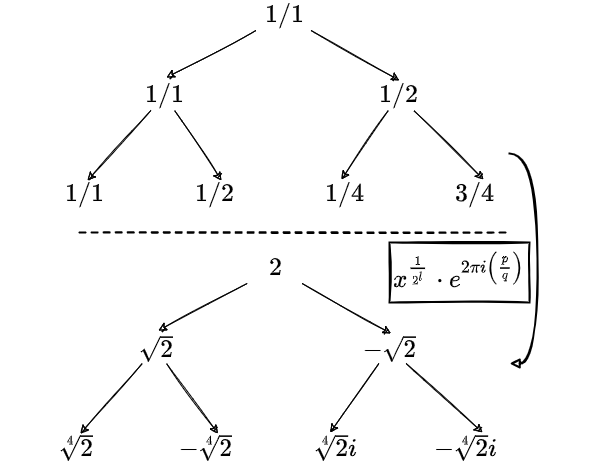
\includegraphics[width=0.8\linewidth]{rational_root_tree.png}
  \caption{The upper tree depicts the steps of \textsc{\textsc{Circle\_Roots\_Rational\_Form}}($p,q,l$) in Alg.\ref{alg:circ_roots_rational_form} for $l=2$, $p=1$, and $q=1$. The lower tree depicts the steps of \textsc{Roots}($r,t,u,l$) in Alg.\ref{alg:roots} for $r=2$, $l=2$, $p=1$, and $q=1$}\label{fig:rat_roots_tree}
\end{figure}

\begin{figure}[h]
  \centering
  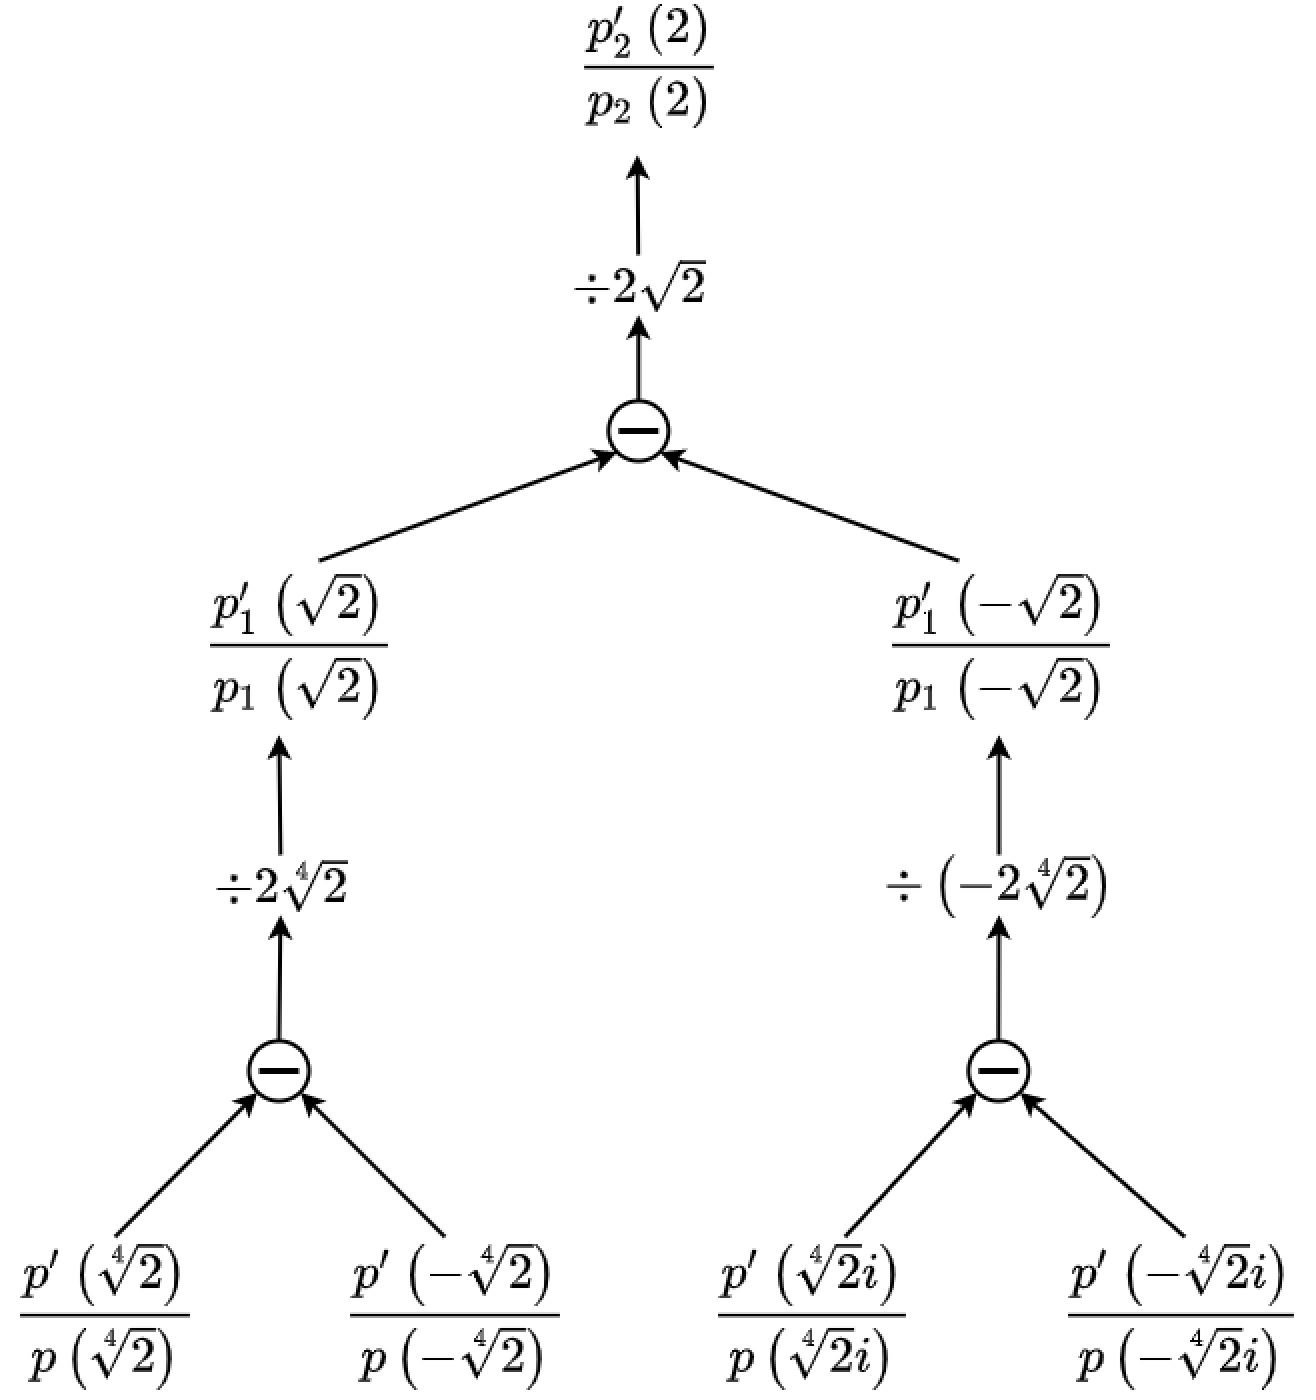
\includegraphics[width=0.8\linewidth]{p_prime.png}
  \caption{The steps of \textsc{DLG\_Rational\_Form}($p,p^\prime,r,t,u,l$) in Alg.\ref{alg:DLG_rational_form} for $r=2$, $l=2$, $t=1$, and $u=1$.}\label{fig:DLG}
\end{figure}

In this section we present the design of the general algorithm for approximating the root radius given by Eq.~\ref{eqdndrt0}.
There are two main steps: 1) going down the rational root tree, \emph{i.e.,} performing Alg.~\ref{alg:circ_roots_rational_form}, and 2) going up the rational root tree, \emph{i.e.,} performing Alg.~\ref{alg:DLG_rational_form}.
The going-down is depicted in Fig.~\ref{fig:rat_roots_tree} and the going-up is depicted in Fig.~\ref{fig:DLG}.
The other procedures are simple bookkeeping/preprocessing steps in between the two main going-down/going-up steps.
In particular we
1) first convert a complex number $x$ into polar coordinates $r,\theta$ where $\theta \approx \frac{p}{q} = \frac{p}{2^\epsilon}$, \emph{i.e.,} perform Alg.~\ref{alg:rational_angle_approx},
2) perform the first going-down pass which gives the rational angles for the roots of $x$ in fraction form, \emph{i.e.,} perform Alg.~\ref{alg:circ_roots_rational_form},
3) perform the second pass of the going-down algorithm where we compute the values $|x|^{\frac{1}{2^m}} \exp(2 \pi i \frac{p}{q})$ at the $m^\mathrm{th}$ level, and
4) finally compute the values given by Eq.~\ref{eqdndrt} going back up the rational root tree.

\begin{algorithm}
   \caption{\textsc{Circle\_Roots\_Rational\_Form}($p,q,l$)}
   \label{alg:circ_roots_rational_form}
\begin{algorithmic}
\IF{ $p\%q$ == 0}
  \STATE  $r, s$ := (1,1)
\ELSE
  \STATE  $r, s$ := ($p$,$2q$)
\ENDIF
  \IF{ r\%s == 0}
    \STATE $t, u$ := (1,2)
  \ELSE
    \STATE $t, u$ := $(2r+s, 2s)$
  \ENDIF
	  \IF{$l$ == 1}
		  \RETURN [($r,s$),($t,u$)]
	\ELSIF {$l$ != 0}
		\STATE left  := \textsc{Circle\_Roots\_Rational\_Form}($r,s,l-1$)
		\STATE right := \textsc{Circle\_Roots\_Rational\_Form}($t,u,l-1$)
		\RETURN left $\cup$ right
	\ELSE
		\RETURN  [($p,q$)]
      \ENDIF
\end{algorithmic}
\end{algorithm}

The intuition behind Alg.~\ref{alg:circ_roots_rational_form} is that the square root operation satisfies
\begin{equation}\label{eq:rat_sq_imag}
p \% q \neq  0 \implies   \sqrt{\exp \left(2 \pi i \frac{p}{q}\right)}  = \exp \left(2 \pi i \frac{p}{2q}\right)
\end{equation}
and
\begin{equation}\label{eq:rat_sq_real}
p \% q = 0 \implies   \sqrt{\exp \left(2 \pi i \frac{1}{1}\right)}  = \exp \left(2 \pi i \frac{1}{1}\right) = 1,
\end{equation}
and the negation operation satisfies
\begin{equation}\label{eq:rat_neg_imag}
p \% q \neq  0 \implies   -\exp \left(2 \pi i \frac{r}{s}\right)  = \exp \left(2 \pi i \frac{2r+s} {2s}\right)
\end{equation}
and
\begin{equation}\label{eq:rat_neg_real}
p \% q = 0 \implies   \sqrt{\exp \left(2 \pi i \frac{1}{1}\right)}  = \exp \left(2 \pi i \frac{1}{2}\right) = -1;
\end{equation}
therefore, the first four lines of Alg.~\ref{alg:circ_roots_rational_form} compute the (angle of the) positive square root, $\sqrt{x}$, of complex number on the unit circle and the next four lines Alg.~\ref{alg:circ_roots_rational_form} computes the (angle of the) negative square root, $-\sqrt{x}$. Therefore, we have:
\begin{theorem}\label{thm:rat_root_correctness}
  For a complex number $x$ with a rational angle $\frac{p}{q}$, \emph{i.e.,} $x = |x|\exp \left(2 \pi i \frac{p}{q}\right)$, Alg.~\ref{alg:circ_roots_rational_form} correctly computes the roots in Eq.~\ref{eqdndrt}. In particular, for a rational angle in fractional form, it does so with exact precision.
\end{theorem}
\begin{proof}
Equations \ref{eq:rat_sq_imag}, \ref{eq:rat_sq_real}, \ref{eq:rat_neg_imag}, and \ref{eq:rat_neg_real} give the base case and the theorem follows by a straightforward induction.
\end{proof}

Alg. \ref{alg:roots} and Alg. \ref{alg:rational_angle_approx} are both straightforward, so for the rest of this section we focus on the intuition behind Alg.~\ref{alg:DLG_rational_form}.

\begin{algorithm}
\caption{\textsc{Roots}($r,t,u,l$)}
\label{alg:roots}
\begin{algorithmic}
\STATE root\_tree = \textsc{Circle\_Roots\_Rational\_Form}($p,q,l$)
\STATE circ\_root = [$\exp\left(2\cdot\pi\cdot i \cdot \frac{r}{s}\right)$ for $r,s$ in root\_tree]
% \STATE circ\_root       = circ\_roots($t,u,l$)
\STATE roots =[$\sqrt[2^l]{r}\cdot$root for root in circ\_root]
\RETURN roots
\end{algorithmic}
\end{algorithm}


% \begin{algorithm}
%    \caption{circ\_roots\_rational\_form($p,q,l$)}
%    \label{alg:circ_roots_rational_form}
% \begin{algorithmic}
%   \STATE $r, s$  := angle\_sq\_root($p,q$)
% 	\STATE $t, u$  := angle\_neg($r,s$)
% 	  \IF{$l$ == 1}
% 		  \RETURN [($r,s$),($t,u$)]
% 	\ELSIF {$l$ != 0}
% 		\STATE left  := circ\_roots\_rational\_form($r,s,l-1$)
% 		\STATE right := circ\_roots\_rational\_form($t,u,l-1$)
% 		\RETURN left $\cup$ right
% 	\ELSE
% 		\RETURN  [($p,q$)]
%       \ENDIF
% \end{algorithmic}
% \end{algorithm}


% \begin{algorithm}
% \caption{angle\_sq\_root(p,q)}
% \label{alg:angle_sq_root}
% \begin{algorithmic}
% 	\IF{ $p\%q$ == 0}
% 		\RETURN  (1,1)
% 	\ELSE
% 		\RETURN  ($p$,$2q$)
%   \ENDIF
% \end{algorithmic}
% \end{algorithm}
%
%
% \begin{algorithm}
% \caption{angle\_neg(p,q)}
% \label{alg:angle_neg}
% \begin{algorithmic}
% 	\IF{ p\%q == 0}
% 		\RETURN  (1,2)
% 	\ELSE
% 		\RETURN  $(2p+q, 2q)$
%   \ENDIF
% \end{algorithmic}
% \end{algorithm}




% \begin{algorithm}
% \caption{circ\_roots($p,q,l$):}
% \label{alg:circ_roots}
% \begin{algorithmic}
% \STATE roots = circ\_roots\_rational\_form($p,q,l$)
% \RETURN [$\exp\left(2\cdot\pi\cdot i \cdot \frac{r}{s}\right)$ for r,s in roots]
% \end{algorithmic}
% \end{algorithm}





% \clearpage

\begin{algorithm}
\caption{\textsc{DLG\_Rational\_Form}($p,p^\prime,r,t,u,l$)}
\label{alg:DLG_rational_form}
\begin{algorithmic}
\STATE 	root      := \textsc{Roots}($r,t,u,l$)
\FOR {$r_i \in $ root}
\STATE 	base\_step[$i$] := $\frac{p^\prime(r_i)}{p(r_i)}$
\ENDFOR
\STATE  diff[0]   := base\_step
\FOR {$i \leq l$}
\FOR {$j \leq 2^{l-i-1}$}
\STATE 			diff[$i+1$][$j$]:=$\frac{1}{2}\frac{\text{diff}[i][2j]-\text{diff}[i][2j+1]}{\text{root}[2j]}$
\STATE 		root = roots($r,t,u,l-1-i$)
\ENDFOR
\ENDFOR
\RETURN diff$[l][0]$
\end{algorithmic}
\end{algorithm}
Alg. \ref{alg:DLG_rational_form} is a dynamic programming on Equation \ref{eqdndrt}. Therefore, by Thm.~\ref{thm:rat_root_correctness}, we have that Alg.~\ref{alg:DLG_rational_form} correctly computes Eq.~\ref{eqdndrt}.
Specifically, Alg.~\ref{alg:DLG_rational_form} does the following: 1) it computes the last layer of the recursion Eq.~\ref{eqdndrt} (\emph{i.e.,} it computes $p'(x^{\frac{1}{2^l}})/p(x^{\frac{1}{2^l}})$) and then 2) it recursively applies Eq.~\ref{eqdndrt} via dynamic programming until it finally computes $\frac{p_{\ell}'(x)}{p_{\ell}(x)}$ which is the desired quantity.
The former is given by the line ``base\_step[$i$] := $\frac{p^\prime(r_i)}{p(r_i)}$'' and the latter is given by the line ``diff[$i+1$][$j$]:=$\frac{1}{2}\frac{\text{diff}[i][2j]-\text{diff}[i][2j+1]}{\text{root}[2j]}$'' in Alg.~\ref{alg:DLG_rational_form}; the desired output (\emph{i.e.,} $p'(x^{\frac{1}{2^l}})/p(x^{\frac{1}{2^l}})$) is given by the line ``diff$[l][0]$''.




\begin{algorithm}
\caption{\textsc{DLG}($p,p^\prime,l,x, \epsilon$)}
\label{alg:rational_angle_approx}
\begin{algorithmic}
\STATE angle     := $\frac{1}{2\pi i} \log (x)$
\STATE $u $    := $2^{\epsilon}$
\STATE$t$      :=  $(\text{angle} \cdot u)\% 1$
\STATE $r$      := $|x|$
\RETURN \textsc{DLG\_Rational\_Form}($p,p^\prime,r,t,u,l$)
\end{algorithmic}
\end{algorithm}

%
% u     = pod(2,epsilon)
% t     = mp.fmod(angle,pod(2,-epsilon))
% r     = mpf(mp.fabs(x))




% def DLG_rational_form(p,dp,r,t,u,l):
% 	root       = roots(r,t,u,l)
% 	base_step  = [dp(r)*np.reciprocal(p(r)) for r in root]
% 	derivs     = [base_step]
% 	for i in range(l):
% 		derivs.append([])
% 		for j in range(2**(l-i-1)):
% 			derivs[i+1].append((np.reciprocal(root[2*j])/2)*(derivs[i][2*j] - derivs[i][2*j+1]))
% 		root = roots(r,t,u,l-1-i)
% 	return derivs[l][0]

The final step in the algorithm is to use Alg. \ref{alg:rational_angle_approx} to compute root radius approximations $r_d$ and $r_1$.
The procedure is given by Alg.~\ref{alg:DLG_Root_Radius}.
\begin{algorithm}
\caption{\textsc{DLG\_Root\_Radius}($p,p^\prime,p_\mathrm{rev},p^\prime_\mathrm{rev},l, \epsilon, \epsilon' $)}
\label{alg:DLG_Root_Radius}
\begin{algorithmic}
\STATE Uniformly Randomly Generate $x $ in the unit circle
\STATE $d$ := deg($p$)
\STATE $r_\mathrm{min} $ := $d/$\textsc{DLG}($p,p^\prime ,l,x\cdot 2^{-\epsilon}, \epsilon'$)
\STATE $r_\mathrm{max} $ := \textsc{DLG}($p_\mathrm{rev},p^\prime _\mathrm{rev},l,x\cdot 2^{-\epsilon}, \epsilon'$)$/d$
\end{algorithmic}
\end{algorithm}
The rationale for generating a random $x$ is that there may be roots close to 0 and thus, by taking the limit in certain directions, we avoid these possible poles; in particular, we have that
\begin{equation}\label{eq:lim_DLG}
  \lim_{ \epsilon',\epsilon \to \infty }  \textsc{DLG}(p,p^\prime ,l,x\cdot 2^{-\epsilon'}, \epsilon ) = \frac{p_{{\ell}}'(0)}{p_{\ell}(0)}=\Big(\frac{p_{\ell-1}'(x)}{p_{\ell-1}(x)}\Big)_{x=0}'=\Big(\frac{p'(x)}{p(x)}\Big)_{x=0}^{(\ell)},
\end{equation}
for any $x$, if $p(0) \neq 0$ (See Thm~\ref{thm:lim_correctness}).





\section{Theoretical Analysis}
\label{sec:the_ana}
% \newpage
% \clearpage
% \begin{lemma}
% The (relative) condition number operator satisifies the following properties:
% \begin{enumerate}
%   \item $\kappa\{f\} (x) = |x \log'(f(x)) |$
%   \item $\kappa\{f-g\}(x) = |x \frac{ \kappa \{f\}(x)- \kappa \{g\}(x) }{f(x)-g(x)}| $
%   \item $\kappa \left\{\frac{f}{g}\right\} (x)= ||\kappa\{ f\} (x)| - |\kappa\{ g\} (x)||$
%   \item $\kappa \left\{ f \circ g \right\}(x) = \left| |\kappa\{f\} (g(x) )\cdot \kappa\{g\} (x)|\right| $
% \end{enumerate}
% \end{lemma}
% \begin{theorem}
%   The condition number for $\frac{p_l'}{p_l}$ using
% \end{theorem}
We now give some theoretical guarantees: Thm. \ref{thm:lim_correctness} proves the correctness of Alg.~\ref{alg:DLG_Root_Radius}, and Thm. \ref{thm:float_ops} and Thm. \ref{thm:ints} give computational complexity bounds.

\subsection{Correctness of the output}
\begin{theorem}\label{thm:lim_correctness}
 If $p(0) \neq 0$, then Alg. \ref{alg:DLG_Root_Radius} computes the bounds given by Eq.~\ref{eqrtrdbndsrev1}  with probability 1.
\end{theorem}
\begin{proof}
By Lem.~\ref{lem:lim_correctness} we have that the limit in Eq.~\ref{lem:lim_correctness} is well defined. Since there are at most finitely many roots for $p_\ell$ with a high probability Alg.~\ref{alg:DLG_Root_Radius} computes the correct approximation to the bounds in Eq.~\ref{eqrtrdbndsrev1}.
\end{proof}

\subsection{Complexity}
\begin{theorem}\label{thm:float_ops}
Alg. \ref{alg:DLG_rational_form} performs $q $ floating point subtractions, divisions, and multiplications and $q $ applications of $\sin$ and $\cos$, where $q = 2^l$; furthermore, Alg. \ref{alg:DLG_rational_form} performs at most $Cq $  integer additions, ``multiplications-by-2'', and $ \%2^\epsilon $ (\emph{i.e.,} mod $ 2^\epsilon $) operations, where $C=1,3,2$ respectively.
\end{theorem}
\begin{proof}
Looking at Fig.~\ref{fig:rat_roots_tree} and Fig.~\ref{fig:DLG}, we can see that the computational tree for the Alg.~\ref{alg:DLG_rational_form} is a binary tree with $2^l = q$ nodes; the proof for the constants $C=1,3,2$ follows similarly follows from the inspection of the operations performed in Alg.~\ref{alg:circ_roots_rational_form}.
\end{proof}

\begin{theorem}\label{thm:ints}
The $Cq $  integer additions, ``multiplications-by-2'', and $ \%2^\epsilon $ (\emph{i.e.,} mod $ 2^\epsilon $) operations in Alg.~\ref{alg:DLG_rational_form} have negligible overhead. More precisely, integer additions are always additions of 2 $\epsilon \log \ell $-bit integers and ``multiplications-by-2'' and $ \%2^\epsilon $ (\emph{i.e.,} mod $ 2^\epsilon $) operations have constant time overhead.
\end{theorem}

\begin{proof}
  Since Alg.~\ref{alg:rational_angle_approx} always passes in a denominator which is a power of two all of the integer $\%$ and $\cdot$ operations are in fact ``multiplications-by-2'', and $ \%2^\epsilon $ (\emph{i.e.,} mod $ 2^\epsilon $) operations by a straightforward proof similar to the one in Alg.~\ref{alg:DLG_rational_form}. Thus these operation are essentially constant overhead bit shift operations on a computing machine with binary words. Since $p\% r$ always reduces $p \mapsto 1$, we have that whenever an overflow of more than $\log r$-bits happens in Alg.~\ref{alg:circ_roots_rational_form} it gets converted to an $\log r$-bit integer; therefore, it suffices to prove that $\log r$ is bounded by  $\epsilon \log \ell $. However, this once again follows by induction on the binary computation tree: since this tree has depth $\ell$ we see that any denominator is bounded by $\epsilon \log \ell $ by a simple induction.
\end{proof}

In order to prove Thm.~\ref{thm:lim_correctness} we must first prove Lem.~\ref{lem:lim_correctness}.
\begin{lemma}\label{lem:lim_correctness}
   If $p(0) \neq 0$, then the limit $   \lim_{ x \to 0 }  \textsc{DLG}(p,p^\prime ,l,x )$ is always well-defined.
   \end{lemma}
\begin{proof}
By applying induction on Eq. \ref{eqdnd}, we have that $p_l(0) \neq 0$ if $p(0) \neq 0$, and thus it suffices to consider the behavior of the numerator in  Eq.~\ref{eqdndrt}. The case $\ell = 1$ follows from an application of L'Hopital's rule. For $\ell \neq 1$, there are two cases: either $\sqrt x~$ divides the numerator of $\frac{p_{\ell}'(\sqrt x~)}{p_{\ell}(\sqrt x~)}$ or it does not. If it does, then we are done since we can once again apply L'Hopital's rule. Otherwise, we get that $p_{\ell}'(\sqrt x~) = c_0+c_1\sqrt x~ + ... +c_k(\sqrt x~)^k$ for some $c_i$ with $c_0 \neq 0$. But then we have
\begin{align*}
\begin{split}
\frac{p_{\ell+1}'(\sqrt x~)}{p_{\ell+1}(\sqrt x~)}
&= \frac{1}{2\sqrt x}\Big(\frac{p_{\ell}'(\sqrt x~)}{p_{\ell}(\sqrt x~)}-\frac{p_{\ell}'(-\sqrt x~)}{p_{\ell}(-\sqrt x~)}\Big) \\
%& = \frac{1}{2\sqrt x}\frac{b_0c_0 + \sqrt x \cdot N(\sqrt x) - b_0c_0 - \sqrt x \cdot N'(\sqrt x)}{p_{\ell}'(\sqrt x~)p_{\ell}'(-\sqrt x~)}\\
& = \frac{1}{2\sqrt x}\frac{b_0c_0 + \sqrt x \cdot N_1(\sqrt x) - b_0c_0 - \sqrt x \cdot N_2(\sqrt x)}{p_{\ell}'(\sqrt x~)p_{\ell}'(-\sqrt x~)}\\
& = \frac{1}{2}\frac{  N_1(\sqrt x) -  N_2(\sqrt x)}{p_{\ell}'(\sqrt x~)p_{\ell}'(-\sqrt x~)},
\end{split}
\end{align*}
 for some polynomials $N_1$ and $N_2$ with $b_0 = p_{\ell}'(0)$. Therefore the limit at zero is once again well-defined.
\end{proof}
\subsection{Stability}

\begin{definition}
If $\tilde f$is an algorithm for computing $f$ we let $\delta f(x) = f(x) - \tilde f (x)$ then the condition number of $\tilde \{ f\} (x)$ at $x$,  $\kappa \{\tilde f\} (x)$ , is given by
$$ \kappa  \{\tilde f\} (x) = \lim _{\varepsilon \rightarrow 0}\,\sup _{\|\delta x\|\,\leq \,\varepsilon }{\frac {\|\delta f(x)\|}{\|\delta x\|}}.
$$
\end{definition}

\begin{lemma}
The (relative) condition number operator $\kappa$ satisfies the following properties:
\begin{enumerate}
  \item $\kappa\{f\} (x) = |x \log'(f(x)) |$
  % \item $\kappa\{f-g\}(x) = |x \frac{ \kappa \{f\}(x)- \kappa \{g\}(x) }{f(x)-g(x)}| $
  \item $\kappa \left\{\frac{f}{g}\right\} (x)= ||\kappa\{ f\} (x)| - |\kappa\{ g\} (x)||$
    \item $\kappa \{x^ d \} (x)= d$
  % \item $\kappa \left\{ f \circ g \right\}(x) = \left| |\kappa\{f\} (g(x) )\cdot \kappa\{g\} (x)|\right| $
\end{enumerate}
\end{lemma}
\begin{proof}
This follows from the definition of the condition number.
\end{proof}
\begin{theorem}\label{thm:stability}
If $p_\ell(0)\neq 0$, then $\frac{p_{\ell}'(x)}{p_{\ell}(x)}$ is well-conditioned at any point sufficiently close to 0.
\end{theorem}
\begin{proof}
  The proof of Lem.~\ref{lem:lim_correctness} gives us that $\frac{p_{\ell}'(x)}{p_{\ell}(x)}$ is a well behaved rational function at any point close to zero and thus the condition number $\kappa\{\frac{p_{\ell}'}{p_{\ell}}\}(x)$ is well defined at this point since the condition number of arithmetic operations of functions are themselves arithmetic operations in those same functions and the conditions number for a polynomial of degree $d \in \mathbb{R}$ is exactly $d$; therefore, $\kappa\{\frac{p_{\ell}'}{p_{\ell}}\}(x)$ has a well defined/bounded condition number in the limit to zero.
\end{proof}

\begin{remark}
Even though Thm.~\ref{thm:stability} states that $\frac{p_{\ell}'(x)}{p_{\ell}(x)}$ is highly stable, in practice, computating this function requires the use of trigonometric functions (\emph{i.e.,} the roots in Alg.~\ref{alg:roots}); therefore, our added precision in Alg..~\ref{alg:circ_roots_rational_form} helps with the instability associated with Alg.~\ref{alg:roots}. Intuitively this helps the instability because the trigonometric functions are the only subroutines in the algorithm that have a non constant condition number and thus, special care must be taken with them; in particular, our algorithm gives a precise value (up to user specified precision) of the angle arguements to these trigonometric functions.
\end{remark}


\section{Experimental Results}
\label{sec:exp}
\subsection{Setup}
%what are the polynomials used?
We now present the results of our experiments in which we compute the bounds on the extremal root radii $|x_1|$ and $|x_d|$ given by \ref{eqrtrdbndsrev1} for the polynomials in the test suite of MPSolve. The test suite covers a number of univariate polynomial families over a range of degrees. (A fuller description of the test suite can be found in \texttt{https://numpi.dm.unipi.it/mpsolve-2.2/mpsolve.pdf}.)

Given a polynomial $p(x)$ of degree $d$, we use an implementation of DLG iterations that incorporates our algorithm from Section \ref{sec:alg_des} for computing $(p'(x)/p(x))^{(\ell)}$ and in turn compute bounds, or estimates, for root radii, $r_1 = r_{\text{max}}$ and $r_d = r_{\text{min}}$ given by (\ref{eqrtrdbndsrev1}) on extremal root radii $|x_1|$ and $|x_d|$, respectively. The performance of these bounds are evaluated on the \emph{relative error} in comparison to the corresponding root radius computed by MPSolve. That is,
$$
\text{relative error}(r_i) = \frac{\big|r_i - |x_i|\big|}{|x_i|},~i = 1, d,
$$
where $|x_i|$ is the minimal or maximal root radius found using MPSolve and $r_i$ is the corresponding estimate for the root radii we compute.

%explain the choices for l and e
For the parameters, we use $\ell = \lfloor \log_2 d \rfloor$ and for the precision we emperically found that
$
% \begin{equation*}
e =  2^{\ell/3} + 330
% \end{equation*}
$
bits of precision behaved pretty well; however, deducing the theoritically correct values of $e$ would be an interesting future research direction.

By choosing $\mathcal{O}(\log d)$ iterations, we keep the number of iterations relatively small even when the degree of the polynomial increases. For instance, $\ell = 6$ for $d = \deg(p(x)) = 100$, and when $d$ grows to 6400, we still have $\ell = 12$; likewise, since the number of bits of precision used where $e = 2^{\mathcal{O}(\ell)} = \mathcal{O}(d)$, we have that the precision did not grow too large neither.

All experiments were performed using Python 3.7.7 and MPSolve 3.2.1 on MacOS 11.6.1 with 2.8 GHz Dual-Core Intel Core i5 with 8 GB memory.
% How challenging are these polyomials?

\subsection{Observations}
% how good are these results?
The overall results support our claims that our root radii approximations perform well when $p(x)$ has no roots extremely close to zero whereas the estimates are poor otherwise. The test results for the \texttt{chebyshev} family of polynomials in Table \ref{tab:chebyshev} demonstrate this trend quite clearly.

In general, the relative errors for the minimal root radius $|x_d|$ is 1.0 or less for roots away from the origin by more than 0.01, with some notable exceptions such as $p(x)  = x^d - h^d$. That is, the difference between the minimal root radius bound we compute and the absolute value of the smallest root $x_d$ tends to be less than $|x_d|$, i.e., $|r_d - |x_d|| \leq |x_d|$. Combined with the bound given in (\ref{eqratio0}) gives us a rough heuristic expectation that $|x_d| \leq r_d \leq 2|x_d|$ if $|x_d| > 0.01$.

The relative errors for the maximal root radius $|x_1|$ for the lower bound $r_1$ reflects a similar trend: The errors are close to 1 when $|x_1|$ is large, showing that in relation to the root radius, our estimate is close to 0, the worst lower bound possible. Since $1/x_1$ the smallest root of $p_{\text{rev}}$, this is essentially the same situation as the root $x_d$ of $p(x)$ being near 0.

Finally, our results demonstrate the consequence of Thm. \ref{eqratiorcp} in Table \ref{tab:nroots} showing the figures for polynomial family \texttt{nroots} of the form $p(x)  = x^d - 1$. The ratio of $|p(0)/p'(0)|$ is infinite, so our algorithm estimates the minimal root radius to be much larger than the actual root radius. On the other hand, the algorithm estimates the maximal root radius to be close to 0 since $|p_{\text{rev}}(0)/p_{\text{rev}}'(0)|$ = 0.

\subsection{Tables}
The columns of the tables, in order, are respectively:
% \begin{itemize}
$d$: degree of the input polynomial,
$\ell$: number of iterations,
$e$: $-\log(|x|)$,
mp.dps: the \texttt{mpmath} precision level used,
the relative errors for the minimum and maximum root radii,
total runtime,
the extremal root radii as computed by MPSolve for the particular given polynomial.
% \end{itemize}

 The entries `-' in the tables indicate the test was terminated before completion.


\begin{table}
\vskip -0.1775in
\caption{Experimental Data for \texttt{chebyshev}} % Chebyshev}
\vskip -0.15in\label{tab:chebyshev}
\vskip -0.0000005in
\begin{center}
\begin{small}
\begin{sc}
\begin{tabular}{rccccccc}
\toprule
&  &  & mp.-& relative  & relative & run- & mpsolve \\
$d~$& $\ell$& $e$ & dps&error $r_d$       & error $r_1$ &time& root radius\\
\midrule
 20 & 4 & 616 & 332 & 0.155 & 0.0939 & 0.27 & $[0.0785, 0.997]$\\
 40 & 5 & 616 & 332 & 0.0981 & 0.0589 & 1.13 & $[0.0393, 0.999]$\\
 80 & 6 & 617 & 334 & 0.0593 & 0.0353 & 5.26 & $[0.0196, 1.0]$\\
 160 & 7 & 617 & 334 & 2.71 & 0.0205 & 20.88 & $[0.00982, 1.0]$\\
 320 & 8 & 617 & 334 & 37.6 & 0.465 & 88.4 & $[0.00491, 1.0]$\\
\bottomrule
\end{tabular}
\end{sc}
\end{small}
\end{center}
\vskip -0.15in
\vskip 0.073in \end{table}

\begin{table}
\vskip -0.1775in
\caption{Experimental Data for \texttt{chrma}} %  chromatic polynomial (zero root removed) kind a}
\vskip -0.15in\label{tab:chrma}
\vskip -0.0000005in
\begin{center}
\begin{small}
\begin{sc}
\begin{tabular}{rccccccc}
\toprule
&  &  & mp.-& relative  & relative & run- & mpsolve \\
$d~$& $\ell$& $e$ & dps&error $r_d$       & error $r_1$ &time& root radius\\
\midrule
 21 & 4 & 616 & 332 & 0.215 & 0.139 & 0.22 & $[1.0, 3.17]$\\
 85 & 6 & 617 & 334 & 0.0369 & 0.0452 & 5.63 & $[1.0, 3.25]$\\
 341 & 8 & 617 & 334 & 0.717 & 0.547 & 105.48 & $[0.884, 3.41]$\\
\bottomrule
\end{tabular}
\end{sc}
\end{small}
\end{center}
\vskip -0.15in
\vskip 0.073in \end{table}


\begin{table}
\vskip -0.1775in
\caption{Experimental Data for \texttt{chrma\_d}} % chromatic polynomial deflated: a}
\vskip -0.15in\label{tab:chrma_d}
\vskip -0.0000005in
\begin{center}
\begin{small}
\begin{sc}
\begin{tabular}{rccccccc}
\toprule
&  &  & mp.-& relative  & relative & run- & mpsolve \\
$d~$& $\ell$& $e$ & dps&error $r_d$       & error $r_1$ &time& root radius\\
\midrule
20 & 4 & 616 & 332 & 0.16 & 0.175 & 0.26 & $[1.3, 3.01]$\\
 84 & 6 & 617 & 334 & 0.0548 & 0.00507 & 5.53 & $[1.1, 3.06]$\\
 340 & 8 & 617 & 334 & 0.658 & 0.699 & 93.82 & $[0.741, 3.11]$\\
\bottomrule
\end{tabular}
\end{sc}
\end{small}
\end{center}
\vskip -0.15in
\vskip 0.073in \end{table}


\begin{table}
\vskip -0.1775in
\caption{Experimental Data for \texttt{chrmc}} %  chromatic polynomial (zero root removed) kind c}
\vskip -0.15in\label{tab:chrmc}
\vskip -0.0000005in
\begin{center}
\begin{small}
\begin{sc}
\begin{tabular}{rccccccc}
\toprule
&  &  & mp.-& relative  & relative & run- & mpsolve \\
$d~$& $\ell$& $e$ & dps&error $r_d$  & error $r_1$ &time& root radius\\
\midrule
 22 & 4 & 616 & 332 & 0.211 & 0.138 & 0.3 & $[1.0, 3.03]$\\
 342 & 8 & 617 & 334 & 0.718 & 0.279 & 94.64 & $[0.897, 4.13]$\\
\bottomrule
\end{tabular}
\end{sc}
\end{small}
\end{center}
\vskip -0.15in
\vskip 0.073in \end{table}


\begin{table}
\vskip -0.1775in
\caption{Experimental Data for \texttt{chrmc\_d}} % chromatic polynomial deflated, kind c}
\vskip -0.15in\label{tab:chrmc_d}
\vskip -0.0000005in
\begin{center}
\begin{small}
\begin{sc}
\begin{tabular}{rccccccc}
\toprule
&  &  & mp.-& relative  & relative & run- & mpsolve \\
$d~$& $\ell$& $e$ & dps&error $r_d$       & error $r_1$ &time& root radius\\
\midrule
11 & 3 & 616 & 332 & 0.251 & 0.242 & 0.05 & $[1.27, 2.8]$\\
 43 & 5 & 616 & 332 & 0.101 & 0.0996 & 1.23 & $[1.02, 2.97]$\\
 171 & 7 & 617 & 334 & 0.268 & 1.13 & 22.05 & $[0.715, 3.07]$\\
 683 & 9 & 619 & 338 & 0.164 & 0.257 & 374.69 & $[0.519, 3.1]$\\
\bottomrule
\end{tabular}
\end{sc}
\end{small}
\end{center}
\vskip -0.15in
\vskip 0.073in \end{table}


\begin{table}
\vskip -0.1775in
\caption{Experimental Data for \texttt{curz}} % Curz}
\vskip -0.15in\label{tab:curz}
\vskip -0.0000005in
\begin{center}
\begin{small}
\begin{sc}
\begin{tabular}{rccccccc}
\toprule
             &  &  & mp.-& relative  & relative & run- & mpsolve \\
$d~$& $\ell$& $e$ & dps&error $r_d$       & error $r_1$ &time& root radius\\
\midrule
 20 & 4 & 616 & 332 & 0.156 & 0.854 & 0.21 & $[0.452, 1.15]$\\
 40 & 5 & 616 & 332 & 0.199 & 0.776 & 1.13 & $[0.379, 1.26]$\\
 80 & 6 & 617 & 334 & 0.086 & 0.227 & 5.49 & $[0.318, 1.34]$\\
 160 & 7 & 617 & 334 & 0.0385 & 0.509 & 20.79 & $[0.271, 1.38]$\\
\bottomrule
\end{tabular}
\end{sc}
\end{small}
\end{center}
\vskip -0.15in
\vskip 0.073in \end{table}


\begin{table}
\vskip -0.1775in
\caption{Experimental Data for \texttt{easy}} % Easy}
\vskip -0.15in\label{tab:easy}
\vskip -0.0000005in
\begin{center}
\begin{small}
\begin{sc}
\begin{tabular}{rccccccc}
\toprule
&  &  & mp.-& relative  & relative & run- & mpsolve \\
$d~$& $\ell$& $e$ & dps&error $r_d$       & error $r_1$ &time& root radius\\
\midrule
 100 & 6 & 617 & 334 & 0.12 & 0.0809 & 6.35 & $[0.949, 0.98]$\\
 200 & 7 & 617 & 334 & 0.068 & 0.047 & 25.57 & $[0.971, 0.99]$\\
 400 & 8 & 617 & 334 & 0.0381 & 0.0265 & 104.47 & $[0.983, 0.995]$\\
 1600 &10& 619 & 338 & 0.01 & 0.00 & 2228.22 & $[0.995, 0.999]$\\ %old nonmemo version data
  3200 &11& 619 & 338 & 0.00 & - & - & $[0.997, 0.999]$\\ %did not finish
\bottomrule
\end{tabular}
\end{sc}
\end{small}
\end{center}
\vskip -0.15in
\vskip 0.073in \end{table}


\begin{table}
\vskip -0.1775in
\caption{Experimental Data for \texttt{exp}} % Exp}
\vskip -0.15in\label{tab:exp}
\vskip -0.0000005in
\begin{center}
\begin{small}
\begin{sc}
\begin{tabular}{rccccccc}
\toprule
&  &  & mp.-& relative  & relative & run- & mpsolve \\
$d~$& $\ell$& $e$ & dps&error $r_d$       & error $r_1$ &time& root radius\\
\midrule
 50 & 5 & 616 & 332 & 3.76 & 0.126 & 1.48 & $[14.9, 39.4]$\\
100 & 6 & 617 & 334 & 0.367 & 0.0598 & 7.37 & $[28.9, 83.9]$\\
 200 & 7 & 617 & 334 & 0.714 & 0.839 & 28.22 & $[56.8, 176.0]$\\
 400 & 8 & 617 & 334 & 0.965 & 0.985 & 107.96 & $[113.0, 365.0]$\\
\bottomrule
\end{tabular}
\end{sc}
\end{small}
\end{center}
\vskip -0.15in
\vskip 0.073in \end{table}

\begin{table}
\vskip -0.1775in
\caption{Experimental Data for \texttt{geom1}} % Geom1}
\vskip -0.15in\label{tab:geom1}
\vskip -0.0000005in
\begin{center}
\begin{small}
\begin{sc}
\begin{tabular}{rccccccc}
\toprule
&  &  & mp.-& relative  & relative & run- & mpsolve \\
$d~$& $\ell$& $e$ & dps&error $r_d$       & error $r_1$ &time& root radius\\
\midrule
 10 & 3 & 616 & 332 & 0.334 & 0.25 & 0.05 & $[1.0, 1.0\text{e+}18]$\\
 15 & 3 & 616 & 332 & 0.403 & 1.0 & 0.08 & $[1.0, 1.0\text{e+}28]$\\
 20 & 4 & 616 & 332 & 0.206 & 1.0 & 0.28 & $[1.0, 1.0\text{e+}38]$\\
 40 & 5 & 616 & 332 & 0.122 & 1.0 & 1.18 & $[1.0, 1.0\text{e+}78]$\\
\bottomrule
\end{tabular}
\end{sc}
\end{small}
\end{center}
\vskip -0.15in
\vskip 0.073in \end{table}

\begin{table}
\vskip -0.1775in
\caption{Experimental Data for \texttt{geom2}} % Geom2}
\vskip -0.15in\label{tab:geom2}
\vskip -0.0000005in
\begin{center}
\begin{small}
\begin{sc}
\begin{tabular}{rccccccc}
\toprule
&  &  & mp.-& relative  & relative & run- & mpsolve \\
$d~$& $\ell$& $e$ & dps&error $r_d$       & error $r_1$ &time& root radius\\
\midrule
 10 & 3 & 616 & 332 & 0.334 & 0.25 & 0.06 & $[1.0\text{e-}18, 1.0]$\\
 15 & 3 & 616 & 332 & 8.09e+4 & 0.287 & 0.06 & $[1.0\text{e-}28, 1.0]$\\
 20 & 4 & 616 & 332 & 2.63e+26 & 0.171 & 0.23 & $[1.0\text{e-}38, 1.0]$\\
 40 & 5 & 616 & 332 & 1.61e+72 & 0.109 & 1.14 & $[1.0\text{e-}78, 1.0]$\\
\bottomrule
\end{tabular}
\end{sc}
\end{small}
\end{center}
\vskip -0.15in
\vskip 0.073in \end{table}

\begin{table}
\vskip -0.1775in
\caption{Experimental Data for \texttt{geom3}} % Geom3}
\vskip -0.15in\label{tab:geom3}
\vskip -0.0000005in
\begin{center}
\begin{small}
\begin{sc}
\begin{tabular}{rccccccc}
\toprule
&  &  & mp.-& relative  & relative & run- & mpsolve \\
$d~$& $\ell$& $e$ & dps&error $r_d$       & error $r_1$ &time& root radius\\
\midrule
 10 & 3 & 616 & 332 & 0.334 & 0.25 & 0.05 & $[9.54\text{e-}7, 0.25]$\\
 20 & 4 & 616 & 332 & 2.41 & 0.171 & 0.24 & $[9.09\text{e-}13, 0.25]$\\
 40 & 5 & 616 & 332 & 1.95e+18 & 0.109 & 1.15 & $[8.27\text{e-}25, 0.25]$\\
 80 & 6 & 617 & 334 & 1.83e+45 & 0.0662 & 5.73 & $[6.84\text{e-}49, 0.25]$\\
\bottomrule
\end{tabular}
\end{sc}
\end{small}
\end{center}
\vskip -0.15in
\vskip 0.073in \end{table}


\begin{table}
\vskip -0.1775in
\caption{Experimental Data for \texttt{geom4}} % Geom4}
\vskip -0.15in\label{tab:geom4}
\vskip -0.0000005in
\begin{center}
\begin{small}
\begin{sc}
\begin{tabular}{rccccccc}
\toprule
&  &  & mp.-& relative  & relative & run- & mpsolve \\
$d~$& $\ell$& $e$ & dps&error $r_d$       & error $r_1$ &time& root radius\\
\midrule
 10 & 3 & 616 & 332 & 0.334 & 0.25 & 0.05 & $[4.0, 1.05\text{e+}6]$\\
 20 & 4 & 616 & 332 & 0.206 & 0.707 & 0.27 & $[4.0, 1.1\text{e+}12]$\\
 40 & 5 & 616 & 332 & 0.122 & 1.0 & 1.15 & $[4.0, 1.21\text{e+}24]$\\
 80 & 6 & 617 & 334 & 0.0709 & 1.0 & 5.28 & $[4.0, 1.46\text{e+}48]$\\
\bottomrule
\end{tabular}
\end{sc}
\end{small}
\end{center}
\vskip -0.15in
\vskip 0.073in \end{table}

\begin{table}
\vskip -0.1775in
\caption{Experimental Data for \texttt{hermite}} % Hermite}
\vskip -0.15in\label{tab:hermite}
\vskip -0.0000005in
\begin{center}
\begin{small}
\begin{sc}
\begin{tabular}{rccccccc}
\toprule
&  &  & mp.-& relative  & relative & run- & mpsolve \\
$d~$& $\ell$& $e$ & dps&error $r_d$       & error $r_1$ &time& root radius\\
\midrule
 20 & 4 & 616 & 332 & 0.155 & 0.129 & 0.28 & $[0.245, 5.39]$\\
 40 & 5 & 616 & 332 & 0.0981 & 0.0876 & 1.31 & $[0.175, 8.1]$\\
 80 & 6 & 617 & 334 & 0.0593 & 0.0555 & 5.97 & $[0.124, 11.9]$\\
 160 & 7 & 617 & 334 & 0.0348 & 0.0335 & 23.56 & $[0.0877, 17.2]$\\
 320 & 8 & 617 & 334 & 2.08 & 0.785 & 88.88 & $[0.062, 24.7]$\\
\bottomrule
\end{tabular}
\end{sc}
\end{small}
\end{center}
\vskip -0.15in
\vskip 0.073in \end{table}

\begin{table}
\vskip -0.1775in
\caption{Experimental Data for \texttt{kam1}} % Kam1}
\vskip -0.15in\label{tab:kam1}
\vskip -0.0000005in
\begin{center}
\begin{small}
\begin{sc}
\begin{tabular}{rccccccc}
\toprule
&  &  & mp.-& relative  & relative & run- & mpsolve \\
$d$& $\ell$& $e$ & dps&error $r_d$       & error $r_1$ &time& root radius\\
\midrule
 7 & 2 & 615 & 331 & 0.368 & 1.0 & 0.01 & $[3.0\text{e-}12, 15.8]$\\
 7 & 2 & 615 & 331 & 0.368 & 1.0 & 0.01 & $[3.0\text{e-}40, 1.0\text{e+}4]$\\
 7 & 2 & 615 & 331 & 2.37e+93 & 1.0 & 0.01 & $[3.0\text{e-}140, 1.0\text{e+}14]$\\
\bottomrule
\end{tabular}
\end{sc}
\end{small}
\end{center}
\vskip -0.15in
\vskip 0.073in \end{table}

\begin{table}
\vskip -0.1775in
\caption{Experimental Data for \texttt{kam2}} % Kam2}
\vskip -0.15in
\label{tab:kam2}
\vskip -0.0000005in
\begin{center}
\begin{small}
\begin{sc}
\begin{tabular}{rccccccc}
\toprule
&  &  & mp.-& relative  & relative & run- & mpsolve \\
$d$& $\ell$& $e$ & dps&error $r_d$       & error $r_1$ &time& root radius\\
\midrule
 9 & 3 & 616 & 332 & 0.107 & 1.0 & 0.03 & $[1.73\text{e-}6, 251.0]$\\
 9 & 3 & 616 & 332 & 0.107 & 1.0 & 0.03 & $[1.73\text{e-}20, 1.0\text{e+}8]$\\
 9 & 3 & 616 & 332 & 4.23e+46 & 1.0 & 0.03 & $[1.73\text{e-}70, 1.0\text{e+}28]$\\
\bottomrule
\end{tabular}
\end{sc}
\end{small}
\end{center}
\vskip -0.15in
\vskip 0.073in \end{table}

\begin{table}
\vskip -0.1775in
\caption{Experimental Data for \texttt{kam3}} % Kam3}
\vskip -0.15in\label{tab:kam3}
\vskip -0.0000005in
\begin{center}
\begin{small}
\begin{sc}
\begin{tabular}{rccccccc}
\toprule
&  &  & mp.-& relative  & relative & run- & mpsolve \\
$d$& $\ell$& $e$ & dps&error $r_d$       & error $r_1$ &time& root radius\\
\midrule
 9 & 3 & 616 & 332 & 0.107 & 1.0 & 0.03 & $[1.73\text{e-}6, 251.0]$\\
 9 & 3 & 616 & 332 & 0.107 & 1.0 & 0.03 & $[1.73\text{e-}20, 1.0\text{e+}8]$\\
 9 & 3 & 616 & 332 & 4.23e+46 & 1.0 & 0.03 & $[1.73\text{e-}70, 1.0\text{e+}28]$\\
\bottomrule
\end{tabular}
\end{sc}
\end{small}
\end{center}
\vskip -0.15in
\vskip 0.073in \end{table}

\begin{table}
\vskip -0.1775in
\caption{Experimental Data for \texttt{kir1}} % Kir1}
\label{tab:kir1}
\vskip -0.0000005in
\begin{center}
\begin{small}
\begin{sc}
\begin{tabular}{rccccccc}
\toprule
&  &  & mp.-& relative  & relative & run- & mpsolve \\
$d~$& $\ell$& $e$ & dps&error $r_d$       & error $r_1$ &time& root radius\\
\midrule
 8 & 3 & 616 & 332 & 0.000244 & 0.000244 & 0.02 & $[0.5, 0.5]$\\ %symb
 44 & 5 & 616 & 332 & 4.41e-5 & 0.000443 & 1.28 & $[0.5, 0.5]$\\
  84 & 6 & 617 & 334 & 2.29e-5 & 0.000464 & 2.9 & $[0.5, 0.5]$\\
 164 & 7 & 617 & 334 & 1.16e-5 & 0.000476 & 9.79 & $[0.5, 0.5]$\\
\bottomrule
\end{tabular}
\end{sc}
\end{small}
\end{center}
\vskip -0.15in
\vskip 0.073in \end{table}

\begin{table}
\vskip -0.1775in
\caption{Experimental Data for \texttt{kir1\_mod}} % Kir1 mod}
\label{tab:kir1_mod}
\vskip -0.0000005in
\begin{center}
\begin{small}
\begin{sc}
\begin{tabular}{rccccccc}
\toprule
&  &  & mp.-& relative  & relative & run- & mpsolve \\
$d~$& $\ell$& $e$ & dps&error $r_d$       & error $r_1$ &time& root radius\\
\midrule
 44 & 5 & 616 & 332 & 0.000983 & 0.00095 & 1.26 & $[0.5, 0.5]$\\
 84 & 6 & 617 & 334 & 0.00364 & 0.00364 & 2.99 & $[0.498, 0.502]$\\
 164 & 7 & 617 & 334 & 0.00734 & 0.00749 & 10.35 & $[0.496, 0.504]$\\ %_mod
\bottomrule
\end{tabular}
\end{sc}
\end{small}
\end{center}
\vskip -0.15in
\vskip 0.073in \end{table}


\begin{table}
\vskip -0.1775in
\caption{Experimental Data for \texttt{lagurerre}} %  Lagurerre }
\label{tab:lagurerre}
\vskip -0.0000005in
\begin{center}
\begin{small}
\begin{sc}
\begin{tabular}{rccccccc}
\toprule
&  &  & mp.-& relative  & relative & run- & mpsolve \\
$d~$& $\ell$& $e$ & dps&error $r_d$       & error $r_1$ &time& root radius\\
\midrule
 20 & 4 & 616 & 332 & 0.206 & 0.167 & 0.22 & $[0.0705, 66.5]$\\
 40 & 5 & 616 & 332 & 0.122 & 0.108 & 1.28 & $[0.0357, 142.0]$\\
 80 & 6 & 617 & 334 & 0.0709 & 0.0659 & 5.63 & $[0.018, 297.0]$\\
 160 & 7 & 617 & 334 & 3.09 & 0.954 & 22.21 & $[0.00901, 610.0]$\\
 320 & 8 & 617 & 334 & 41.4 & 0.996 & 89.64 & $[0.00451, 1.24\text{e+}3]$\\
\bottomrule
\end{tabular}
\end{sc}
\end{small}
\end{center}
\vskip -0.15in
\vskip 0.073in \end{table}

\begin{table}
\vskip -0.1775in
\caption{Experimental Data for \texttt{lar1}} % Lar1}
\label{tab:lar1}
\vskip -0.0000005in
\begin{center}
\begin{small}
\begin{sc}
\begin{tabular}{rccccccc}
\toprule
&  &  & mp.-& relative  & relative & run- & mpsolve \\
$d~$& $\ell$& $e$ & dps&error $r_d$       & error $r_1$ &time& root radius\\
\midrule
 20 & 4 & 616 & 332 & 7.06e+9 & 1.0 & 0.1 & $[3.73\text{e-}22, 1.0\text{e+}50]$\\
 200 & 7 & 617 & 334 & 9.69e+19 & 0.311 & 0.83 & $[3.73\text{e-}22, 41.0]$\\
\bottomrule
\end{tabular}
\end{sc}
\end{small}
\end{center}
\vskip -0.15in
\vskip 0.073in \end{table}

\begin{table}
\vskip -0.1775in
\caption{Experimental Data for \texttt{legendre}} % Legendre}
\label{tab:legendre}
\vskip -0.0000005in
\begin{center}
\begin{small}
\begin{sc}
\begin{tabular}{rccccccc}
\toprule
&  &  & mp.-& relative  & relative & run- & mpsolve \\
$d~$& $\ell$& $e$ & dps&error $r_d$       & error $r_1$ &time& root radius\\
\midrule
 20 & 4 & 616 & 332 & 0.155 & 0.0969 & 0.25 & $[0.0765, 0.993]$\\
 40 & 5 & 616 & 332 & 0.0981 & 0.0604 & 1.15 & $[0.0388, 0.998]$\\
 80 & 6 & 617 & 334 & 0.0593 & 0.0359 & 6.08 & $[0.0195, 1.0]$\\
  160 & 7 & 617 & 334 & 2.72 & 0.0637 & 19.97 & $[0.00979, 1.0]$\\
 320 & 8 & 617 & 334 & 37.7 & 0.456 & 81.12 & $[0.0049, 1.0]$\\
\bottomrule
\end{tabular}
\end{sc}
\end{small}
\end{center}
\vskip -0.15in
\vskip 0.073in \end{table}

\begin{table}
\vskip -0.1775in
\caption{Experimental Data for \texttt{lsr}} % LSR} %polynomial having roots with very large and very small moduli
\label{tab:lsr}
\vskip -0.0000005in
\begin{center}
\begin{small}
\begin{sc}
\begin{tabular}{rccccccc}
\toprule
&  &  & mp.-& relative  & relative & run- & mpsolve \\
$d~$& $\ell$& $e$ & dps&error $r_d$       & error $r_1$ &time& root radius\\
\midrule
 24 & 4 & 616 & 332 & 2.88e+8 & 1.0 & 0.29 & $[1.0\text{e-}20, 1.0\text{e+}20]$\\
 52 & 5 & 616 & 332 & 1.81e+14 & 1.0 & 0.25 & $[1.0\text{e-}20, 1.0\text{e+}10]$\\ %lsr4_1
 52 & 5 & 616 & 332 & 1.81e+34 & 1.0 & 0.22 & $[1.0\text{e-}40, 1.0\text{e+}20]$\\ %lsr4_2
 52 & 5 & 616 & 332 & 1.81e+74 & 1.0 & 0.2 & $[1.0\text{e-}80, 1.0\text{e+}40]$\\ %lsr4_3
 224 & 7 & 617 & 334 & 3.62e+18 & 1.0 & 9.8 & $[1.0\text{e-}20, 1.0\text{e+}20]$\\
 500 & 8 & 617 & 334 & 1.92e+3 & 1.0 & 6.79 & $[0.0001, 2.0\text{e+}4]$\\
 500 & 8 & 617 & 334 & 5.77e+3 & 0.995 & 3.27 & $[3.33\text{e-}5, 1.0\text{e+}3]$\\
 500 & 8 & 617 & 334 & 1.05 & 1.0 & 3.05 & $[0.0916, 1.0\text{e+}200]$\\
\bottomrule
\end{tabular}
\end{sc}
\end{small}
\end{center}
\vskip -0.15in
\vskip 0.073in \end{table}

\begin{table}
\vskip -0.1775in
\caption{Experimental Data for \texttt{mand}} % Mand}
\label{tab:mand}
\vskip -0.0000005in
\begin{center}
\begin{small}
\begin{sc}
\begin{tabular}{rccccccc}
\toprule
&  &  & mp.-& relative  & relative & run- & mpsolve \\
$d~$& $\ell$& $e$ & dps&error $r_d$       & error $r_1$ &time& root radius\\
\midrule
   31 & 4 & 616 & 332 & 0.295 & 0.144 & 0.4 & $[0.445, 2.0]$\\
   63 & 5 & 616 & 332 & 0.127 & 0.0854 & 2.16 & $[0.403, 2.0]$\\
 127 & 6 & 617 & 334 & 0.0898 & 0.0488 & 8.58 & $[0.373, 2.0]$\\
 255 & 7 & 617 & 334 & 0.0609 & 0.701 & 37.41 & $[0.351, 2.0]$\\
 511 & 8 & 617 & 334 & 0.0234 & 1.63 & 174.71 & $[0.334, 2.0]$\\
1023 & 9 & 619 & 338 & 0.357 & 0.142 & 569.08 & $[0.321, 2.0]$\\
2047 & 10 & 619 & 338 & 1.12 & 0.241 & 2372.57 & $[0.311, 2.0]$\\
4095 & 11 & 619 & 338 & 1.68 & 0.38 & 9209.19 & $[0.303, 2.0]$\\
\bottomrule
\end{tabular}
\end{sc}
\end{small}
\end{center}
\vskip -0.15in
\vskip 0.13in \end{table}



\begin{table}
\vskip -0.1775in
\caption{Experimental Data for \texttt{mig1}} % Mig1}
\label{tab:mig1}
\vskip -0.0000005in
\begin{center}
\begin{small}
\begin{sc}
\begin{tabular}{rccccccc}
\toprule
&  &  & mp.-& relative  & relative & run- & mpsolve \\
$d~$& $\ell$& $e$ & dps&error $r_d$       & error $r_1$ &time& root radius\\
\midrule
 20 & 4 & 616 & 332 & 0.126 & 1.0 & 0.08 & $[0.01, 2.26]$\\
  50 & 5 & 616 & 332 & 0.0157 & 0.987 & 1.8 & $[0.00999, 1.83\text{e+}3]$\\
 100 & 6 & 617 & 334 & 0.0563 & 1.0 & 0.5 & $[0.01, 1.15]$\\
 100 & 6 & 617 & 334 & 0.0183 & 1.0 & 4.05 & $[0.01, 7.92]$\\
 200 & 7 & 617 & 334 & 2.66 & 1.0 & 0.8 & $[0.01, 1.07]$\\
 200 & 7 & 617 & 334 & 2.59 & 0.999 & 9.37 & $[0.01, 2.33]$\\
 500 & 8 & 617 & 334 & 18.2 & 0.99 & 1.59 & $[0.01, 1.03]$\\
 500 & 8 & 617 & 334 & 18.0 & 0.984 & 15.65 & $[0.01, 1.36]$\\ %mig1_500_1
\bottomrule
\end{tabular}
\end{sc}
\end{small}
\end{center}
\vskip -0.15in
\vskip 0.073in \end{table}


\begin{table}
\vskip -0.1775in
\caption{Experimental Data for \texttt{mult}} % Mult}
\label{tab:mult}
\vskip -0.0000005in
\begin{center}
\begin{small}
\begin{sc}
\begin{tabular}{rccccccc}
\toprule
&  &  & mp.-& relative  & relative & run- & mpsolve \\
$d~$& $\ell$& $e$ & dps&error $r_d$       & error $r_1$ &time& root radius\\
\midrule
 15 & 3 & 616 & 332 & 0.29 & 0.189 & 0.12 & $[0.869, 1.07]$\\
 20 & 4 & 616 & 332 & 0.0782 & 0.475 & 0.24 & $[0.01, 2.68]$\\
 22 & 4 & 616 & 332 & 0.213 & 0.105 & 0.24 & $[1.0, 20.0]$\\
  68 & 6 & 617 & 334 & 0.0566 & 0.0556 & 4.59 & $[0.25, 2.24]$\\
\bottomrule
\end{tabular}
\end{sc}
\end{small}
\end{center}
\vskip -0.15in
\vskip 0.073in \end{table}


\begin{table}
\vskip -0.1775in
\caption{Experimental Data for \texttt{nroots}} % $x^n - 1$}
\label{tab:nroots}
\vskip -0.0000005in
\begin{center}
\begin{small}
\begin{sc}
\begin{tabular}{rccccccc}
\toprule
&  &  & mp.-& relative  & relative & run- & mpsolve \\
$d~$& $\ell$& $e$ & dps&error $r_d$       & error $r_1$ &time& root radius\\
\midrule
 50 & 5 & 616 & 332 & 5.18e+13 & 1.0 & 0.12 & $[1.0, 1.0]$\\
 100 & 6 & 617 & 334 & 7.06e+6 & 1.0 & 0.19 & $[1.0, 1.0]$\\
 200 & 7 & 617 & 334 & 2.69e+3 & 1.0 & 0.39 & $[1.0, 1.0]$\\
 400 & 8 & 617 & 334 & 50.5 & 0.981 & 0.79 & $[1.0, 1.0]$\\
 800 & 9 & 619 & 338 & 6.34 & 0.864 & 1.73 & $[1.0, 1.0]$\\
 1600 & 10 & 619 & 338 & 1.71 & 0.631 & 3.19 & $[1.0, 1.0]$\\
 3200 & 11 & 619 & 338 & 0.645 & 0.392 & 6.79 & $[1.0, 1.0]$\\
 6400 & 12 & 623 & 346 & 0.289 & 0.224 & 14.55 & $[1.0, 1.0]$\\
\bottomrule
\end{tabular}
\end{sc}
\end{small}
\end{center}
\vskip -0.15in
\vskip 0.073in \end{table}

\begin{table}
\vskip -0.1775in
\caption{Experimental Data for \texttt{nrooti}} % $x^n - i$}
\label{tab:nrooti}
\vskip -0.0000005in
\begin{center}
\begin{small}
\begin{sc}
\begin{tabular}{rccccccc}
\toprule
&  &  & mp.-& relative  & relative & run- & mpsolve \\
$d~$& $\ell$& $e$ & dps&error $r_d$       & error $r_1$ &time& root radius\\
\midrule
 50 & 5 & 616 & 332 & 4.94e+13 & 1.0 & 0.1 & $[1.0, 1.0]$\\
 100 & 6 & 617 & 334 & 7.07e+6 & 1.0 & 0.32 & $[1.0, 1.0]$\\
  200 & 7 & 617 & 334 & 2.69e+3 & 1.0 & 0.46 & $[1.0, 1.0]$\\
 400 & 8 & 617 & 334 & 50.5 & 0.981 & 0.85 & $[1.0, 1.0]$\\
 800 & 9 & 619 & 338 & 6.34 & 0.864 & 1.85 & $[1.0, 1.0]$\\
 1600 & 10 & 619 & 338 & 1.71 & 0.631 & 3.23 & $[1.0, 1.0]$\\
 3200 & 11 & 619 & 338 & 0.645 & 0.392 & 7.02 & $[1.0, 1.0]$\\
 6400 & 12 & 623 & 346 & 0.289 & 0.224 & 13.31 & $[1.0, 1.0]$\\
\bottomrule
\end{tabular}
\end{sc}
\end{small}
\end{center}
\vskip -0.15in
\vskip 0.073in \end{table}

\begin{table}
\vskip -0.1775in
\caption{Experimental Data for \texttt{sendra}} %  Sendra}
\label{tab:sendra}
\vskip -0.0000005in
\begin{center}
\begin{small}
\begin{sc}
\begin{tabular}{rccccccc}
\toprule
&  &  & mp.-& relative  & relative & run- & mpsolve \\
$d~$& $\ell$& $e$ & dps&error $r_d$       & error $r_1$ &time& root radius\\
\midrule
 20 & 4 & 616 & 332 & 0.283 & 0.158 & 0.25 & $[0.9, 2.05]$\\
 40 & 5 & 616 & 332 & 0.159 & 0.101 & 1.25 & $[0.95, 2.02]$\\
 80 & 6 & 617 & 334 & 0.287 & 0.573 & 5.2 & $[0.975, 2.01]$\\
 160 & 7 & 617 & 334 & 0.658 & 2.14 & 24.34 & $[0.987, 2.01]$\\
 320 & 8 & 617 & 334 & 0.809 & 1.64 & 88.08 & $[0.994, 2.0]$\\
\bottomrule
\end{tabular}
\end{sc}
\end{small}
\end{center}
\vskip -0.15in
\vskip 0.073in \end{table}

\begin{table}
\vskip -0.1775in
\caption{Experimental Data for \texttt{sparse}}
\label{tab:sparse}
\vskip -0.0000005in
\begin{center}
\begin{small}
\begin{sc}
\begin{tabular}{rccccccc}
\toprule
&  &  & mp.-& relative  & relative & run- & mpsolve \\
$d~$& $\ell$& $e$ & dps&error $r_d$       & error $r_1$ &time& root radius\\
\midrule
100 & 6 & 617 & 334 & 0.11 & 1.0 & 0.26 & $[0.968, 1.01]$\\
 200 & 7 & 617 & 334 & 0.0361 & 0.995 & 1.16 & $[0.969, 1.0]$\\
 400 & 8 & 617 & 334 & 0.0211 & 0.929 & 2.19 & $[0.969, 1.0]$\\
 800 & 9 & 619 & 338 & 0.0118 & 0.739 & 6.56 & $[0.969, 1.0]$\\
  6400 & 12 & 623 & 346 & 0.00202 & 0.158 & 72.81 & $[0.969, 1.0]$\\
\bottomrule
\end{tabular}
\end{sc}
\end{small}
\end{center}
\vskip -0.15in
\vskip 0.073in \end{table}

\begin{table}
\vskip -0.1775in
\caption{Experimental Data for \texttt{spiral}} %  Spiral}
\label{tab:spiral}
\vskip -0.0000005in
\begin{center}
\begin{small}
\begin{sc}
\begin{tabular}{rccccccc}
\toprule
&  &  & mp.-& relative  & relative & run- & mpsolve \\
$d~$& $\ell$& $e$ & dps&error $r_d$       & error $r_1$ &time& root radius\\
\midrule
 10 & 3 & 616 & 332 & 5.1e-7 & 1.21e-6 & 0.05 & $[1.0, 1.0]$\\
 15 & 3 & 616 & 332 & 3.49e-7 & 1.15e-6 & 0.07 & $[1.0, 1.0]$\\
 20 & 4 & 616 & 332 & 4.55e-7 & 1.3e-6 & 0.23 & $[1.0, 1.0]$\\
 25 & 4 & 616 & 332 & 3.67e-7 & 1.25e-6 & 0.29 & $[1.0, 1.0]$\\
 30 & 4 & 616 & 332 & 3.08e-7 & 1.21e-6 & 0.41 & $[1.0, 1.0]$\\
\bottomrule
\end{tabular}
\end{sc}
\end{small}
\end{center}
\vskip -0.15in
\vskip 0.073in \end{table}




\begin{table}
\vskip -0.1775in
\caption{Experimental Data for \texttt{toep}} % Toeplitz}
\label{tab:toep}
\vskip -0.0000005in
\begin{center}
\begin{small}
\begin{sc}
\begin{tabular}{rccccccc}
\toprule
&  &  & mp.-& relative  & relative & run- & mpsolve \\
$d~$& $\ell$& $e$ & dps&error $r_d$       & error $r_1$ &time& root radius\\
\midrule
 128 & 7 & 617 & 334 & 0.0386 & 0.562 & 18.71 & $[1.31, 64.4]$\\
 256 & 8 & 617 & 334 & 0.0219 & 0.918 & 73.35 & $[1.34, 64.4]$\\
 128 & 7 & 617 & 334 & 0.0386 & 0.0272 & 17.68 & $[0.4, 13.2]$\\
 256 & 8 & 617 & 334 & 0.0225 & 0.599 & 72.66 & $[0.383, 13.2]$\\
\bottomrule
\end{tabular}
\end{sc}
\end{small}
\end{center}
\vskip -0.15in
\vskip 0.073in \end{table}


\begin{table}
\vskip -0.1775in
\caption{Experimental Data for \texttt{wilk}} % Wilk}
\label{tab:wilk}
\vskip -0.0000005in
\begin{center}
\begin{small}
\begin{sc}
\begin{tabular}{rccccccc}
\toprule
&  &  & mp.-& relative  & relative & run- & mpsolve \\
$d~$& $\ell$& $e$ & dps&error $r_d$       & error $r_1$ &time& root radius\\
\midrule
 20 & 4 & 616 & 332 & 0.206 & 0.141 & 0.22 & $[1.0, 20.0]$\\
 30 & 4 & 616 & 332 & 0.237 & 0.0859 & 0.33 & $[1.0, 319.0]$\\
 40 & 5 & 616 & 332 & 0.122 & 0.0927 & 1.27 & $[1.0, 40.0]$\\
 80 & 6 & 617 & 334 & 0.0709 & 0.121 & 5.59 & $[1.0, 80.0]$\\
 160 & 7 & 617 & 334 & 0.0404 & 0.824 & 21.82 & $[1.0, 160.0]$\\
 320 & 8 & 617 & 334 & 0.0228 & 0.983 & 89.77 & $[1.0, 320.0]$\\
\bottomrule
\end{tabular}
\end{sc}
\end{small}
\end{center}
\vskip -0.15in
\vskip 0.073in \end{table}



%%
%% The acknowledgments section is defined using the "acks" environment
%% (and NOT an unnumbered section). This ensures the proper
%% identification of the section in the article metadata, and the
%% consistent spelling of the heading.
% \begin{acks}
% To Robert, for the bagels and explaining CMYK and color spaces.
% \end{acks}

%%
%% The next two lines define the bibliography style to be used, and
%% the bibliography file.
\bibliographystyle{splncs04}
\bibliography{ref.bib}

%%
%% If your work has an appendix, this is the place to put it.
\appendix





\end{document}
